\documentclass[a4paper,11pt]{scrreprt}\usepackage[]{graphicx}\usepackage[]{color}
%% maxwidth is the original width if it is less than linewidth
%% otherwise use linewidth (to make sure the graphics do not exceed the margin)
\makeatletter
\def\maxwidth{ %
  \ifdim\Gin@nat@width>\linewidth
    \linewidth
  \else
    \Gin@nat@width
  \fi
}
\makeatother

\definecolor{fgcolor}{rgb}{0.345, 0.345, 0.345}
\newcommand{\hlnum}[1]{\textcolor[rgb]{0.686,0.059,0.569}{#1}}%
\newcommand{\hlstr}[1]{\textcolor[rgb]{0.192,0.494,0.8}{#1}}%
\newcommand{\hlcom}[1]{\textcolor[rgb]{0.678,0.584,0.686}{\textit{#1}}}%
\newcommand{\hlopt}[1]{\textcolor[rgb]{0,0,0}{#1}}%
\newcommand{\hlstd}[1]{\textcolor[rgb]{0.345,0.345,0.345}{#1}}%
\newcommand{\hlkwa}[1]{\textcolor[rgb]{0.161,0.373,0.58}{\textbf{#1}}}%
\newcommand{\hlkwb}[1]{\textcolor[rgb]{0.69,0.353,0.396}{#1}}%
\newcommand{\hlkwc}[1]{\textcolor[rgb]{0.333,0.667,0.333}{#1}}%
\newcommand{\hlkwd}[1]{\textcolor[rgb]{0.737,0.353,0.396}{\textbf{#1}}}%
\let\hlipl\hlkwb

\usepackage{framed}
\makeatletter
\newenvironment{kframe}{%
 \def\at@end@of@kframe{}%
 \ifinner\ifhmode%
  \def\at@end@of@kframe{\end{minipage}}%
  \begin{minipage}{\columnwidth}%
 \fi\fi%
 \def\FrameCommand##1{\hskip\@totalleftmargin \hskip-\fboxsep
 \colorbox{shadecolor}{##1}\hskip-\fboxsep
     % There is no \\@totalrightmargin, so:
     \hskip-\linewidth \hskip-\@totalleftmargin \hskip\columnwidth}%
 \MakeFramed {\advance\hsize-\width
   \@totalleftmargin\z@ \linewidth\hsize
   \@setminipage}}%
 {\par\unskip\endMakeFramed%
 \at@end@of@kframe}
\makeatother

\definecolor{shadecolor}{rgb}{.97, .97, .97}
\definecolor{messagecolor}{rgb}{0, 0, 0}
\definecolor{warningcolor}{rgb}{1, 0, 1}
\definecolor{errorcolor}{rgb}{1, 0, 0}
\newenvironment{knitrout}{}{} % an empty environment to be redefined in TeX

\usepackage{alltt}



\let\oldLaTeX\LaTeX
\renewcommand{\LaTeX}{\textrm{\oldLaTeX}}


\usepackage{scrhack}
\usepackage{makeidx}
  \makeindex
\usepackage{booktabs}
\usepackage{float}
\usepackage{geometry}
\usepackage{graphicx}
\usepackage{lmodern}
\usepackage{microtype}
\usepackage[utf8]{inputenc}
\usepackage[T1]{fontenc}
\usepackage{tabularx}
\usepackage{listings}
\usepackage{lstautogobble}
\usepackage{xcolor}
\usepackage{longtable}
\definecolor{Orange}{HTML}{F68B33}
\definecolor{DarkOrange}{HTML}{D4582A}
\usepackage{bold-extra}
\lstset{
language=[LaTeX]TeX,
basicstyle=\ttfamily,
commentstyle=\color{black!60}\ttfamily,
texcsstyle=*\color{blue},
moretexcs={setlength,chapter,subsection,subsubsection,appendix,addbibresource,FloatBarrier,contentspage,units,includegraphics,noteswithsource,notes,source,bottomrule,midrule,toprule,footcite,footcites,textcite,textcites,Chapref,topref,Vref,Cref},
columns=flexible,
breaklines=true,
backgroundcolor=\color{black!5},
literate={~} {\(\sim\)}{1},
moredelim = [is][\slshape\color{violet}]{@@}{@@},
classoffset=1,
morekeywords={grattan}, keywordstyle = \color{Orange}\bfseries, 
classoffset=0,
escapechar={\^*}{*}
}
\usepackage{fancyvrb}
\newcommand{\nverb}[1]{
\begin{Verbatim}
 #1
\end{Verbatim}

}

\RedeclareSectionCommand[tocnumwidth=2em]{chapter}
\RedeclareSectionCommand[tocnumwidth=2.5em, tocindent=2em]{section}
\RedeclareSectionCommand[tocindent=4.7em]{subsection}

\lstdefinelanguage{BibTeX}
  {keywords={%
      @Article,@book,@collectedbook,@conference,@electronic,@ieeetranbstctl,%
      @inbook,@incollectedbook,@incollection,@injournal,@inproceedings,%
      @manual,@mastersthesis,@misc,@patent,@periodical,@phdthesis,@preamble,%
      @proceedings,@standard,@string,@TechReport,@unpublished%
      },
   comment=[l][\itshape]{@comment},
   sensitive=false,
   autogobble=true,
   keywordstyle = \color{red}\bfseries,
   moredelim = [is][\slshape\color{violet}]{@@}{@@},
  }

\usepackage{bbding}

\usepackage{upquote}  % for `` ''%

\usepackage[justification=justified, singlelinecheck=false, position=above]{caption}
\captionsetup[table]{belowskip=5pt}

% \usepackage{titlesec}     % for customizing sections
% % customize section
% \titleformat{\section}%
%   {\Large\sffamily\bfseries}% format
%   {\makebox[0pt][r]{\thesection\hspace{12pt}}}% label
%   {0pt}% horizontal sep
%   {}% title
% \titleformat{\subsection}%
%   {\large\sffamily\bfseries}% format
%   {\makebox[0pt][r]{\thesubsection\hspace{12pt}}}% label
%   {0pt}% horizontal sep
%   {}% title
% \titleformat{\subsubsection}%
%   {\sffamily\bfseries}% format
%   {\makebox[0pt][r]{\thesubsubsection\hspace{12pt}}}% label
%   {0pt}% horizontal sep
%   {}% title
\renewcommand\sectionlinesformat[4]{%
  \makebox[0pt][r]{#3}#4%
}

\usepackage{varioref}
\usepackage[colorlinks, urlcolor=blue, linkcolor=blue]{hyperref}
\usepackage{cleveref}

% For previous page for 'varioref'
% space after second -2 is important here.
\makeatletter
\patchcmd\cref@old@@vpageref
{\advance\@tempcnta-2}
{\advance\@tempcnta-2 }{\typeout{patch ok}}{\ERRORpatchFaild}
\makeatother

\title{{\textrm{Using \LaTeX\ in reports at Grattan}}}
\subtitle{Manual for \texttt{grattex} v1.2.0 and \texttt{grattanReporter} v0.14.0}
\author{Cameron Chisholm \and Hugh Parsonage}

\newcommand{\defi}[1]{\textbf{\textsf{#1}}}
\newcommand{\ie}{\emph{i.e.}}
\newcommand{\eg}{\emph{e.g.}}
\newcommand*{\etc}{\emph{etc}}

\newcommand*{\rationale}[1]{\par\hfill{\small\itshape\raise1.5ex\hbox{#1}}\vspace{11pt plus 5.5pt}}
\newcommand*{\prereleaseonly}{\marginpar{\footnotesize\lstinline[language=R]!pre_release!}}
\newcommand*{\releaseonly}{\marginpar{\footnotesize\lstinline[language=R]!release!}}

\newcommand*{\fromversion}[1]{\marginpar{\footnotesize From v#1}}

\usepackage{realboxes}
\usepackage{manfnt}

\def\smallstrut{\relax\ifmmode\copy\smallstrutbox\else\unhcopy\strutbox\fi}
\makeatletter
\setbox\strutbox\hbox{%
  \vrule\@height0.5ex % orig .7
        \@depth0\baselineskip
        \@width\z@}%
\makeatother

\newcommand{\code}[1]{\fcolorbox{gray!10}{gray!10}{\smallstrut\texttt{#1}}}
\newcommand{\Code}[1]{\Colorbox{gray!10}{\lstinline!#1!}}
\newcommand{\Codee}[1]{\Colorbox{gray!10}{#1}}

\usepackage{enumitem}

\usepackage{tikz}
  \usetikzlibrary{shapes,arrows}

% Define block styles
\tikzstyle{decision} = [
    rectangle, 
    draw, 
    fill=Orange, 
    text width=4.5em, 
    text badly centered, 
    node distance=3cm, 
    inner sep=0pt ]

\tikzstyle{block} = [
  rectangle, 
  draw, 
  text width=5em, 
  text centered, 
  rounded corners, 
  minimum height=4em]

\tikzstyle{stop} = [
  rectangle, 
  draw, 
  fill=red, 
  text width=5em, 
  text centered, 
  rounded corners, 
  minimum height=4em]

\tikzstyle{line} = [draw, -latex']

\tikzstyle{ok} = [
    ellipse,
    draw,  
    fill=green, 
    node distance=3cm,
    minimum height=2em]
\IfFileExists{upquote.sty}{\usepackage{upquote}}{}
\begin{document}

\maketitle
\tableofcontents
\newpage 
% \subsection*{Interpreting code examples}
% \addcontentsline{toc}{subsection}{Interpreting code examples}
\addsec{Interpreting code examples}
Example code are written using a listing:
\begin{lstlisting}
LaTeX code with some \markup.  
\begin{environment}

\end{environment}
\end{lstlisting}
or inline: \lstinline!\TeX{}!.

Code examples can be, for want of better terms, \emph{complete} or \emph{illustrative}. \defi{Complete} code means the code should be copied-and-pasted directly into the input file without modification, whereas \defi{illustrative} code should be modified based on the desired output. For example, if an author wishes to increase the gap between columns in the overview by 2\,mm, the code excerpt below is complete. The author should copy and paste the following, placing it before \lstinline!\begin{overview}!:
\begin{lstlisting}
\newlength{\overviewextra}
\setlength{\overviewextra}{2mm}
\addtolength{\columnsep}{\overviewextra}
\end{lstlisting}
Whereas in an illustrative version of the above, the author is offered a choice for the gap between columns. In illustrative code examples, such options are coloured violet, slanted, and delimited with chevrons:
\begin{lstlisting}
\newlength{\overviewextra}
\setlength{\overviewextra}{@@<extra column width>@@}
\addtolength{\columnsep}{\overviewextra}
\end{lstlisting}


Text coloured blue is simply syntax highlighting and has no special meaning. All \TeX{} documents are written in plain text (although your text editor/\textsc{IDE} may offer or display similar syntax highlighting). 

\newpage
\chapter{The name of the game}
\LaTeX\ is technically a package of the 1978 computer programme \TeX. 
The language used by your computer to set the words on the page is called \TeX; the \emph{engine} used to convert this to a pdf is called pdf\TeX, and the language you write in is called \LaTeX. 

\TeX\ was written -- recursively -- in order to typeset its own user manual.\footnote{Knuth, D. (1984) \textit{The \TeX book}, Addison-Wesley Professional.} 

In all cases, the \TeX{} is pronounced \(\tau\epsilon\chi\), similar to \emph{tech-} as in \emph{technology} but the X is pronounced as a voiceless velar fricative, like the final sound in \emph{loch} or \emph{Bach}. 

Your interface in which you write \LaTeX\ is called an IDE (integrated development environment). The particular IDE we recommend is called ShareLaTeX, which is an online SaaS provider of \LaTeX. 

\newpage

 \chapter{Some principles for erstwhile MS Word users}
 Learning \LaTeX{} as an MS Word user is a frustrating, confusing, rewarding, and ecstatic experience.  There are some principles that are inviolate for novices.
 \begin{enumerate}
  \item Don't worry about the appearance of your document as your write. Write what you mean. MS Word is a What You See Is What You Get editor. \LaTeX\ is a What You See Is What You \emph{Mean}.
  \item \LaTeX\ takes an author's input and sets out the document's appearance using the author's raw input, the author's advice about how the document should look, and a set of parameters and algorithms that govern tradeoffs concerning document appearance. 
  \item The \verb=grattan.cls= template is designed so that authors do not have to make any layout or typographic decisions.
  \item \LaTeX\ is a butler, not a robot. It may not do exactly as you say, but it will do what you mean. When it doesn't, it either means 
  \begin{itemize}
   \item You've given it a nonsensical instruction
   \item Your instruction contradicts another instruction
   \item Your instruction contravenes good typographic design, as it sees fit
  \end{itemize}

  \item \LaTeX\ is a butler, not a slave: it is a partner in document preparation. In general, your responsibilities should not overlap: you decide the content and it decides the form. Where your responsibilities do overlap, you should seek to \emph{advise} \LaTeX, not to \emph{order} it. Further, you should be as gentle as possible with your advice. Only forcefully advise when the document will not require amendments and you are sure \LaTeX\ is wrong. 
  \item \LaTeX\ is a computer program, not a human. Despite the previous points, there are limits to what \LaTeX\ can do. In particular, \LaTeX\ cannot reword paragraphs. If you ask for five figures and a box to appear on one page, no software can save you. The lesson is not that \LaTeX\ is limited (though it does have weaknesses\footnote{See \url{http://tex.stackexchange.com/questions/27440/what-cant-tex-do} and \url{http://tex.stackexchange.com/questions/70901/typesetting-limitations-of-latex?noredirect=1&lq=1}.}) but that changing the actual words, charts, etc you give it can have a dramatic effect on appearance. 
  \item Don't manually position figures, tables, or boxes. Let them float in the document. It is nearly certain that the initial placement will be odd. As long you have used a \verb=figure=, \verb=table= or \verb=*box= environment, they will float into good positions. For errant figures, tables, or boxes, wait until the document is completely finished before advising positions.
  \item Don't do any of the following:
  \begin{enumerate}
   \item Insert horizontal or vertical whitespace, including manual line-breaks (except in tables)
   \item page- or column-breaking
  \end{enumerate}
  \item Do not ignore errors (\emph{i.e.}~things that prevent compilation). Any errors which you can't resolve in less than 60 seconds should be referred to Cameron Chisholm or Hugh Parsonage. Preferably attach what you think caused the error.
  \item Take note of warnings from time to time. Warnings relating to bibliographies should be fixed immediately. Other warnings are typically just hints that manual intervention may improve the layout -- resolving them can be deferred.

  \item Beware special characters. 
  \begin{table}[h]
   \centering
   \begin{tabular}{ll}
   \toprule
   \textbf{When you want this \dots} & \textbf{\dots type this.} \\
   \midrule
   %
   \$ & \verb=\$= \\
   \% & \verb=\%= \\
   `` & \verb=``= (button above \verb=Tab=) \\
   '' & \verb=''= \\
   \multicolumn{2}{l}{(similarly for single-quotes)} \\ 
   -- (en-dash) & \verb=--=  \\
   --- (em-dash) & \verb=---=  \\
   \(-\) (minus sign) & \verb=\(-\)= \\
   \bottomrule   
  \end{tabular}
  \end{table}

  


  \item The grattan class file assumes your input is encoded in \texttt{UTF-8}. Avoid copying from MS Word to \verb=.tex= files. Otherwise, special characters above will creep in silently. If you must, use \verb=pandoc=.
  \item Use \texttt{\%} for comments.
 \end{enumerate}

 \chapter{Basics of \textrm{\LaTeX}}
 \section{Compilation}
 The process of \LaTeX\ is basically:
 \begin{enumerate}
  \item Start with a plain text file with the file extension \verb=.tex= in a directory/folder
  \item Run the \verb=pdflatex= program on that file. 
  \item The program outputs a pdf file \lstinline!myfile.pdf! or returns an error.
 \end{enumerate}

 In ShareLaTeX, the plain text file is viewed on a browser. The act of pressing the Compile button is equivalent to running \Code{pdflatex} on that file.

 
 \section{Commands and environments}
 \subsection{Commands}
 A \defi{command} starts with a backslash \verb=\= followed by one or more characters.
 The command's \defi{name} is the string of characters after the backslash. 
 A {command} may have zero or more mandatory arguments and zero or more optional arguments. 
 Mandatory arguments are delimited by curly braces; optional arguments by square braces

 \begin{lstlisting}
 \somecommand[@@<optional arg>@@]{@@<mandatory arg1>@@}{@@<mandatory arg2>@@}
 \end{lstlisting} 

 \textbf{\textsf{Note:}} Whitespace after commands with zero arguments is \emph{ignored}. So 

 \begin{lstlisting}
 \LaTeX is a macro package.
 \end{lstlisting}
 
 will typeset: 
\begin{quote}
 \LaTeX is a macro package.
 \end{quote} 
 (Note that there is no space between \LaTeX{} and `is'.)
 On reflection, this is understandable: a command is defined by letters, so a space after a command in effect defines the name.
 But because it's a typesetting program, always having a space would make some things impossible. 
 For example, `This is typed in \LaTeX.' would have a space between \LaTeX{} and the full stop.

 To indicate that a space should follow such a command, use either 

 \begin{lstlisting}
 \LaTeX{} is a macro package.
 \end{lstlisting}
 wherein the use of braces tells the compiler the command name has finished, or 

 \begin{lstlisting}
 \LaTeX\ is a macro package.
 \end{lstlisting}
 Note that \lstinline!\LaTeX\! is not a single command. 
 Rather \lstinline!\LaTeX! is one command; and \Code{\\  } itself is another command that inserts an explicit space. 


 Below is a table of some commands and their arguments:
 
 \begin{table}[H]
 \raggedright
 \renewcommand{\arraystretch}{1.4}
 \newlength{\tabularxlength}
 \setlength{\tabularxlength}{\linewidth}
 \addtolength{\tabularxlength}{0.5\paperwidth}
 \addtolength{\tabularxlength}{-0.5\linewidth}
 \caption{Examples of commands and their arguments}
  \makebox[\textwidth][l]{%
  \begin{tabularx}{\tabularxlength}{lp{2.5cm}X}
    \toprule
    \textbf{\textsf{Command}} & \textbf{\textsf{Arguments}} & \textbf{\textsf{Description}} \\ 
    \midrule
    \verb=\$= & 0 mandatory\newline 0 optional & \textbf{Prints} the \$\ sign\\
    \verb=\textbf= & 1 mandatory\newline 0 optional & Prints its argument in boldface. \\
    \verb=\\= & 0 mandatory\newline 1 optional & Forces a line break, with optional extra space \\
    \verb=\footcite= & 1 mandatory\newline 2 optional & Cites its mandatory argument, with optional pre- or post-notes (such as page numbers) \\
    \verb=\footcites= & $n$ mandatory\newline $2n + 2$ optional & Multiple footcites \\
    \bottomrule
  \end{tabularx}
  }
 \end{table}
 \clearpage
 \subsection{Environments}
 An \defi{environment} looks like
\begin{lstlisting}
  \begin{environment}
   ...
  \end{environment}
\end{lstlisting}
It may have mandatory or optional arguments, which occur immediately after \verb=\begin{environment}=.  

 \begin{table}[h]
 \raggedright
 \renewcommand{\arraystretch}{1.4}
 \setlength{\tabularxlength}{\linewidth}
 \addtolength{\tabularxlength}{0.5\paperwidth}
 \addtolength{\tabularxlength}{-0.5\linewidth}
 \caption{Examples of environments}
  \makebox[\textwidth][l]{%
  \begin{tabularx}{\tabularxlength}{lp{2.5cm}X}
    \toprule
    \textbf{\textsf{Environment}} & \textbf{\textsf{Arguments}} & \textbf{\textsf{Description}} \\ 
    \midrule
    \verb=document= & none & The contents of the document. \\
    \verb=figure= & 1 optional & Creates a section of a document which ``floats'' above the body of the text. Captions and cross-reference labels within a \verb=figure= environment will refer to the figure. The optional argument restricts the placement of the figure on the page. \\ 
    %
    \verb=quote= & none & Used to designate a long quote with additional margin. \\
    %
    \verb=smallbox= & 2 mandatory, 1 optional & Creates a box, limited to one column. The first argument is optional and specifies the position of the box. The second argument is mandatory and specifies the title of the box, the third argument is also mandatory and specifies the cross-reference label of the box. \\ 
    \bottomrule
  \end{tabularx}
  }
  \end{table}
  %

















  \chapter{Drafting a Grattan report}
  \section{Getting started}\label{sec:getting-started}
  To start a Grattan report, working paper, or submission, you can either
  \begin{enumerate}
  \item email Hugh Parsonage, Cameron Chisholm, Andrew McDonald, or Brigitte Phelan and ask to be setup, letting them know:
  \begin{enumerate}
    \item a suitable name for the repository
    \item the contributors 
  \end{enumerate}
  The contributors can be changed after the report is set up. 
  But the repo name cannot. 
  Accordingly, it is important that you choose a name that is evocative of the project, unique, and will have a long shelf-life.
  This can be difficult, and a naming convention has not yet been established; however, names like `HigherEd-report' or `Inquiry-submission' will be rejected---or purged if they slip through.
  \item or, follow the following steps on your own:
    \begin{enumerate}
      \item Visit \url{https://travis-ci.org/HughParsonage/grattex.svg?branch=master} and verify: 
\includegraphics[height=1em]{figure/passing.png}.
      If it shows another image (or no image), please do not proceed.
      \item Login as the `grattaninstitute` super user in \href{https://github.com}{github.com} and \href{https://sharelatex.com}{sharelatex.com}.
      \item Copy \verb=https://github.com/HughParsonage/grattex= to your clipboard
      \item Visit \url{https://github.com/new/import}
      \item Paste \verb=https://github.com/HughParsonage/grattex= into the \verb=Your old repository's clone URL= field.
      \item Choose an evocative name for your repository under \verb=Name=
      \item Select \textbf{Private}
      \item Click \textbf{Begin Import}.
      \item You will be taken to a new page showing import progress. After the import is complete, follow the link which appears.
      \item Click the Settings Tab.

      \makebox[\textwidth][r]{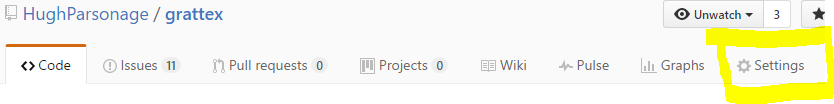
\includegraphics[width=0.9\paperwidth]{figure/github-settings-tab.PNG}}
      \item On the left, click `Collaborators`. 
      \item Add `HughParsonage` and any other authors as desired.
      \item Visit [sharelatex.com](https://sharelatex.com).
      \item Click `New Project > Import from GitHub`.
      \item Locate the repository you just created, and click `Import to ShareLaTeX`. 
      \item If ShareLaTeX fails to compile, this is a bug. Otherwise, proceed. (The first compilation should take several minutes, resulting in a document around 150 pages.)
      \item At the top right, click `Share`.
      \item Add collaborators as desired. 
    \end{enumerate}
  \end{enumerate}
  \section{The preamble}
  The \defi{preamble} is everything outside the \verb=document= environment. (\ie~everything after \verb=\begin{document}=. 
  
  In every \LaTeX\ document, you must have 
  \begin{enumerate}
   \item The \emph{command} \verb=\documentclass= and a valid document class. In our case, use 
   \begin{lstlisting}
\documentclass{grattan}
   \end{lstlisting}
   \item A \verb=document= environment.
  \end{enumerate}
  That is, every \LaTeX\ document must have the following three lines.
  \begin{lstlisting}
\documentclass{@@<style>@@}
  
\begin{document}
  
\end{document}
  \end{lstlisting}




  \subsection{Grattan-specific preamble}
  So that reports look alike, a particular preamble is required that load the Grattan style.
  If you imported the package from GitHub using the instructions in \Vref{sec:getting-started} your report already meets the requirements described below.

  Your preamble must have the following lines.
  \begin{lstlisting}
   \documentclass[@@<options>@@]{grattan}
   
   \title{@@<Title of the report>@@}
   \author{@@<Authors>@@}

   \GrattanReportNumber{@@<number>@@} %% or 
   \GrattanWorkingPaperNumber{@@<number>@@}
   
   \addbibresource{bibliography.bib}
  \end{lstlisting}
  \subsection{Other requirements}
  The \verb=.tex= file must be in a directory containing:
  \begin{enumerate}
   \item The \verb=grattan.cls= file, which creates the document according to the Grattan template.
   \item The \verb=bibliography.bib= file, containing your bibliography database.
   \item The folder \verb=FrontPage= which\releaseonly must contain:
   \begin{enumerate}
    \item A file \verb=FrontPage.pdf=
   \end{enumerate}
   \item The following files (possibly in a subdirectory \verb=logos/=:
    \begin{verbatim}
    aus-gov-logo-stacked-black.pdf
    Bhp.pdf
    GrattanSVGLogo.pdf
    TMF_logo_green-eps-converted-to.pdf
    TMF_logo_green.pdf
    UOM-Pos_S_PMS.pdf
    Vic_Gov_Logo-2016.pdf
    \end{verbatim}


  \end{enumerate}

  \subsection{Class options}
  You can invoke one of the following options by writing 
  \begin{lstlisting}
  \documentclass[@@<options>@@]{grattan}
  \end{lstlisting}
  for example, 
  \begin{lstlisting}
  \documentclass[FrontPage]{grattan}
  \documentclass[FrontPage,continuous]{grattan}
  \end{lstlisting}
  \begin{description}
    \item[embargoed] Issue an embargoed mark on the title page and in the running heads. Enlivens the following commands:
    \begin{enumerate}
      \item \relax\lstinline!\EmbargoDate! The date printed in the embargo fields. By default, \lstinline!XXXX!.
      \item \relax\lstinline!\EmbargoText! The embargo field printed in the running heads and on the title page (unless \lstinline!\EmbargoTitleText! is set). 
      By default \lstinline!Embargoed until 9 pm \EmbargoDate{}!.
      \item \relax\lstinline!\EmbargoTitleText! The text printed on the title page (as distinct from the running heads). By default, \lstinline!\EmbargoText{}!.
    \end{enumerate}
    \item[submission] Document is a submission to inquiries. Omits page 2.
    \item[FrontPage] Use the pdf in the location \lstinline!./FrontPage/FrontPage.pdf! as page 1, rather than a generic one.
    \item[continuous] Use continuous numbering for figures and tables, rather than resetting after each chapter. 
  \end{description}



  
  \section{Frontmatter}
  \subsection{Overview / Summary / Preface}
  Use \index{overview}
  \begin{lstlisting}
   \begin{overview}[-35pt]
    ...
   \end{overview}
  \end{lstlisting}
  for your overview. The \lstinline![-35pt]! is a fudge factor that adjusts the position of the title to vertically balance the overview on the page. It may be abolished in future versions. 
  
  You can also use \lstinline!\begin{summary}! as required. If you want to change the name of the frontmatter, ask us --- it is straight-forward to amend.

  \subsection{Contents page(s)}
  Write \index{contentspage}
  \begin{lstlisting}
   \contentspage
  \end{lstlisting}
  After the \lstinline!overview! environment. This produces a list of figures and a list of boxes. If you don't want some of these lists, again, ask us --- it is straight-forward to omit, but it is a matter for the class file maintainer.
  
  \section{Body text}
  \subsection{Sectioning}
  To start a new chapter, write \index{chapter} \index{section}
  \begin{lstlisting}
   \chapter{@@<chapter title>@@}
  \end{lstlisting}
  Similarly, 
  \begin{lstlisting}
   \chapter{@@<section title>@@}
   \section{@@<subsection title>@@}
   \subsection{@@<subsubsection title>@@}
  \end{lstlisting}
  Title commands increment as expected, except for \lstinline!\subsubsection! which has no counter.
  
  To start an appendix, type \fcolorbox{gray!10}{gray!10}{\lstinline!\\appendix!}.

  \begin{lstlisting}
   \appendix
  \end{lstlisting}

  to mark the end of the main matter and the start of the appendices. Then use \lstinline!\chapter{@@<appendix title>@@}! to title the appendices.
  
  For example:
  \begin{lstlisting}
  \documentclass{grattan}
  
  \title{Brief report}
  \author{Me}
  
  \begin{document}
  
  \begin{overview}
  In this report, we found all is well.
  \end{overview}
  \contentspage
  \chapter{Australia is fine}
  Australia is fine.
  \chapter{How do we know this}
  Grattan analysis of ABS (2016).
  \section{Limitations of analysis}
  Our analysis is wrong.
  
  \chapter{Options for reform}
  Tidy desk.
  \appendix
  \chapter{International comparisons}
  \end{document}
  \end{lstlisting}
  
  \section{Boldface, italics}
  In general, you should write what you \emph{mean}, not what you want displayed. So avoid directly instructing \LaTeX\ to bold or italicize test. Instead, write macros explaining \emph{why} you are using a different font.
  
  That said, you can use \lstinline!\textbf{@@<text>@@}! to make \lstinline!@@<text>@@! boldface and \lstinline!\textit{@@<text>@@}! to make \lstinline!@@<text>@@! italic. You can also use \lstinline!\emph! to \emph{emphasize} text. 
  
  \section{Paragraphs}
  Use a blank line to mark a new paragraph. For example
  \begin{center}
  \begin{minipage}{\textwidth}
  \begin{lstlisting}
   A well-designed GST reform package could support economic growth, make the tax and transfer system more progressive and give state and Commonwealth governments more budgetary options.

   Proposals to extend or broaden Australia's 10 per cent goods and services tax (GST) have been perennial. Current governments face many challenges, such as funding growing healthcare costs, reducing deficits, and cutting inefficient taxes. A higher GST could fund any of these initiatives -- although perhaps not all of them. 
  \end{lstlisting}
  N.B.: The indent here means a continued line. There are only three lines of code illustrated here. 
  \end{minipage}
  \end{center}
  In the above example, \emph{Proposals to extend} will begin on a new paragraph. 

  \subsection{Non-breaking spaces}
  Use \lstinline!~! for a non-breaking space: \lstinline!\$40~million!. 

  Use \Code{\\nobreakdash-} for a non-breaking hyphen: \lstinline!2013\nobreakdash-14!. 



  
  \section{Numbered / bulleted lists}
  Use \verb=enumerate= (for numbered lists) and \verb=itemize= (for bulleted lists) \index{enumerate}\index{itemize}
  \begin{lstlisting}
   \begin{enumerate}
    \item First numbered item
    \item Second numbered item 
    \begin{enumerate}
     \item First item in a nested list
    \end{enumerate}
    \item Third numbered item
   \end{enumerate}

   \begin{itemize}
     \item First bulleted item 
     \item Second bulleted item 
     \begin{itemize}
      \item First nested bulleted item.
     \end{itemize}
   \end{itemize}
  \end{lstlisting}

  
  \section{Floats}
  \subsection{Figures}
  Before you insert a figure, you need to create your image (say in PowerPoint).
  Your file should be saved as a pdf, though almost all image types are supported. 
  If you are going through an external program, ensure the file is moved to the atlas directory of your report. 
  This directory should be placed in the same directory as your \verb=.tex= file.
  
  Once the image is ready, use the following structure to insert a figure.
  \begin{lstlisting}
   \begin{figure}
    \caption{@@<main caption>@@\label{@@<cross-reference key>@@}}%
    \units{@@<secondary caption/y-axis label>@@}
    \includegraphics{atlas/@@image-filename@@}
    \noteswithsource{@@<Notes of the chart>@@}%  
    {@@<Source information>@@}
   \end{figure}
  \end{lstlisting}

  Alternatively, you can save your charts in a single pdf, with each page having a different chart. To refer to the 3rd page in your pack \lstinline!@@<chart-pack-filename.pdf>@@!, use:
  \begin{lstlisting}
  \includegraphics[page=3]{atlas/@@<chart-pack-filename.pdf>@@}
  \end{lstlisting}

  Use \lstinline!\caption! for the boldface caption and \lstinline!\units! for the non-bold (secondary) caption. 
  Use \lstinline!\label! to mark the cross-reference key target, which should be inside the argument to \lstinline!\caption!. 
  
  Use \lstinline!\noteswithsource! to put the notes and source under a figure (or table). Note this command has two mandatory arguments. 
  Use \lstinline!\notes! if you have notes but no source; and \lstinline!\source! if you have a source but no notes. 

  \subsection{Tables}
    Tables are tricky in \LaTeX. Most tables will have the following construction:

    \begin{lstlisting}
    \begin{table}
    \caption{@@<Caption to the table>@@}
   \begin{tabularx}{\columnwidth}{@@<alignment parameters>@@}
    \toprule
    Header1 & Header2 & Header3 \\
    \midrule 
    First row & First row & First row \\
    Second row & Second row & Second row \\
    ...
    Last row & Last row & Last row
    \bottomrule
   \end{tabularx}
   \noteswithsource{@@<Notes>@@}%
   {@@<Source>@@}
   \end{table}
  \end{lstlisting}

  Like with figure, we put the contents of this float in an environment called \Code{table}. 
  The \lstinline!\begin{table}! \dots \lstinline!\end{table}! simply tells \LaTeX{} to float the placement, to use ``Table $N$:'' in the caption, and possibly to note it in the list of tables. 
  It does nothing to actually construct the table.

  The actual construction of the table is handled by \Code{tabularx}\index{tabularx} which is very similar to the standard \Code{tabular} environment. 
  Its first argument is the width of the table and its second argument is the \emph{alignment parameters} of the tabular's columns:

  The \lstinline!@@<alignment parameters>! determine the alignment of the columns, \verb=l= for left-aligned, \verb=c= for centre-aligned, \verb=r= for right-aligned. Others are available. 

  Inside the tabular, use the ampersand \verb=&= to move to the next column and the double-backslash \verb=\\= to move to the next row. 
  Use \verb=\toprule= before the first row, \verb=\bottomrule= after the last row, and \verb=\midrule= to separate the headers from the rest of the table.

\subsection{Excel}
    Most authors would be well-advised to quickly write their tables in Excel and then use Excel2LaTeX.

    To start using Excel2LaTeX:

  \begin{enumerate}
  	\item Go to \url{https://www.ctan.org/pkg/excel2latex?lang=en}
  	\item Download the contents of this package
  	\item Unzip the archive. 
  	\item Enable the add-in for your version of Excel. (\eg~\url{https://support.office.com/en-us/article/Add-or-remove-add-ins-0af570c4-5cf3-4fa9-9b88-403625a0b460})
  	\item Activate the add-in (see Excel documentation for your version).
  	\item Open the Add-Ins tab in Excel, and, with the sheet containing your table open, click \texttt{Convert table to LaTeX}.
  	\item The defaults are usually sensible. Click Copy to clipboard and paste into your \texttt{.tex} source file. 
  \end{enumerate}

  Once you have copied the table, you should make the following adjustments:

  \begin{enumerate}
    \item Use \lstinline!\begin{tabularx}{\linewidth}! instead of 
    \lstinline!\begin{tabular}! (be sure to also change \lstinline!\end{tabular}! to \lstinline!\end{tabularx}!. 

    The \Code{tabularx} environment creates a table of fixed width -- in this case, the current width of the line. 
    It achieves by stretching one or more of the columns.
    The author chooses which columns will be stretchable by replacing the corresponding alignment parameter with \Code{X}.
    \item So you should also change at least one of your columns' alignment parameters to \Code{X}. 
    By default, \Code{X} has a ragged right edge (or is left aligned). 
    \item All \Code{X} columns will stretch to the same width. 
    So if a tabular's natural width is 80\% of the line width, and you replace a single column's alignment parameter with an \Code{X}, then that column will have an extra 20\% of the line width added to its width.
    If, on the other hand, you replace two columns' alignment parameters with \Code{XX}, those columns will each be widened by 10\% of the line width. 
    \item If the column or columns you would like to stretch should be centre-aligned (with both edges ragged), not left-aligned, then instead of putting \Code{X}, you should put \lstinline!>{\centering}X!. 
    If it should have a ragged left edge (be right-aligned), then you should put \lstinline!>{\RaggedLeft}X! or (for a very ragged edge) \lstinline!>{\raggedleft}X!.
\end{enumerate}
  
  
  \subsection*{More advanced} 
  \begin{table}[H]
  \centering
  %\makebox[\textwidth]{%
  \begin{tabular}{rp{9.5cm}}
  \toprule
  \lstinline!\cmidrule(lr){@@<m-n>@@}! & to denote a horizontal rule between the $m$th and $n$th columns. The \verb=(lr)= specifies that the horizontal rule should stop just short of the edges of the columns, to ensure adjacent \verb=\cmidrule=s have a visual breath between them. \\[5pt]
  \lstinline!\multicolumn{@@<n>@@}{@@<al.>@@}{@@<text>@@}! & Puts the \lstinline!@@<text>@@! in a `merged' cell from the current cell across \lstinline!@@<n>@@! columns with horizontal alignment \lstinline!@@<al.>@@! \\
  \bottomrule
  \end{tabular}%
  %}%
  \end{table}

  \subsection{Table styles}
  Rules of thumb:
  \begin{enumerate}
    \item Never use vertical rules in a table.
    \item If a column should be in a particular font, use the array specifier, rather than manually specifying the column. 
    \begin{lstlisting}
    % Wrong:
    \begin{tabularx}{Xl}
    \textbf{State} & Population \\
    \textbf{NSW}   & Very high \\
    \textbf{Vic}   & High\\
    \dots 
    \textbf{Tas}   & Low
    \end{tabularx}

    % OK:
    \begin{tabularx}{>{\bfseries}Xl}
    State & Population \\
    NSW   & Very high \\
    Vic   & High\\
    \dots 
    Tas   & Low
    \end{tabularx}
    \end{lstlisting}
  \end{enumerate}



  \section{Boxes}
  \subsection{smallbox}\index{smallbox}\index{boxes!smallbox}
  Use \verb=\begin{smallbox}= to insert a box intended to fit on one column. There are two mandatory arguments. 

  \begin{lstlisting}
   \begin{smallbox}{@@<title of the box>@@}{box:@@<cross-ref key>@@}
    @@<contents of the box>@@
   \end{smallbox}

  \end{lstlisting}

  \subsection{verysmallbox}\index{verysmallbox}\index{boxes!verysmallbox}
  The very small box is used for boxes which may be sufficiently shorter than a column to share the column with paragraphs from the body text. 
  Such boxes would contain two or fewer paragraphs. 
  
  \subsection{bigbox*} \index{bigbox*}\index{boxes!bigbox*}
  Use \verb=\begin{bigbox*}= to denote a big box.\footnote{The \texttt{*} reflects a convention in \LaTeX\ for a two-column float in an environment name.} The text will flow around the box. 

  \subsubsection*{Figures in boxes must use [H]}
  When you have a figure in a big box, you must use 
  \begin{lstlisting}
   \begin{figure}[H] 
    ...
   \end{figure}
  \end{lstlisting}
  to insert a figure.
  
  Note the \lstinline![H]! which specifies that the figure is to be placed here (or rather, \emph{HERE!}). 
  
  \section{Cross-references}
  There are three \LaTeX{} commands used in cross-referencing: \lstinline!\label!, \lstinline!\Vref! and \lstinline!\Cref!. \index{Vref}\index{Cref}\index{cross-references}\index{label}
  The first designates the target of a cross-reference; the other two are for making a cross-reference to such a target. 

  For example, to refer to some figure, use the following template.

  \begin{lstlisting}
  \Vref{fig:key} shows that ...  

  \begin{figure}
    \caption{The chart's caption\label{fig:key}}
    \includegraphics{thechartfilename.pdf}
  \end{figure}
  \end{lstlisting}

  \lstinline!\Vref{fig:key}! will expand to Figure N shows that ... 

  % \begin{center}
  {{Your labels should be evocative of what is displayed, \emph{not} the number.} }
  {You will end up moving or removing a figure, table, or box and confuse your labels.}
  % \end{center}

  If you refer to a cross-reference that doesn't exist, the pdf will contain a bold \lstinline!??! and the log file will contain a warning.

  If you are referring to a chapter, you must use \lstinline!\Chapref!.

  The contents of \lstinline!\label! can be anything containing letters, underscores, or hyphens. 
  The house style requires the use of the prefixes in \Vref{tbl:prefixes-by-float-type}. 
  Using these prefixes consistently will make auto-completion easier and is necessary for \texttt{grattanReporter} checks. 

  \begin{table}[H]
  \caption{Prefixes to use in cross-reference anchors, by float type\label{tbl:prefixes-by-float-type}}
  \begin{tabular}{>{\ttfamily}l>{\ttfamily}r>{\ttfamily}l}
  \toprule
  \begin{tabular}{@{}p{0.14\linewidth}@{}}
  \textrm{Float}\tabularnewline 
  \textrm{environ.}\tabularnewline 
  \textrm{command}
  \end{tabular} & \textrm{Prefix} & \textrm{Example} \\
  \midrule 
  figure         & fig:       & \verb=\label{fig:prop-hholds-by-decile}= \\
  table          & tbl:       & \verb=\label{tbl:tax-paid-by-bracket}= \\
  box            & box:       & \verb=\begin{smallbox}{A short history of dogs}{box:dogs}= \\
  footnote       & fn:        & \verb=\footnote{A footnote.\label{fn:my-footnote}}= \\
  chapter        & chap:      & \verb=\chapter{Introduction}\label{chap:intro}= \\
  addchap        & chap:      & \verb=\addchap{Or can it}\label{chap:Or-can-it}= \\
  recommendation & rec:       & \verb=\recommendation{Do it}\label{rec:Do-it}= \\
  section        & sec:       & \verb=\section{The budget problem}\label{sec:budget-problem}= \\
  subsection     & subsec:    & \verb=\subsection{Change}\label{subsec:Change}= \\
  subsubsection  & subsubsec: & \verb=\subsubsection{No}\label{subsubsec:No}= \\
  phantomsection & paragraph: & \verb=\phantomsection\label{paragraph:PROP-land-taxes}=\\
  \bottomrule
  \end{tabular}
  \end{table}



  \section{Footnotes and referencing}
  Use the command \lstinline!\footnote! to mark a footnote. Use \lstinline!\textcite! for a citation within a footnote.

  \subsection{Footnotes in boxes}
  Insert footnotes (and \lstinline!\footcite!s) as if they were part of the main body text. 
  The footnotemarks will be letters, not numbers, and the footnote area will be within the box.
  
  \subsection{\texttt{bibliography.bib}}
  The \texttt{bibliography.bib} file is a plain text containing the bibliography databases. The database contains several lines for each entry:
  \begin{lstlisting}[language=BibTeX]
  @@<@type>@@{@@<key>@@,
    author={@@<author name>@@},
    title={@@<title>@@},
    year={@@<year>@@}
  }
  \end{lstlisting}
  There are several elements to a bibliography:
  \begin{enumerate}[leftmargin=5em]
   \item[\texttt{@type}] This specifies the type of reference, such as an article, report, book.
   \item[\texttt{<key>}] This is a string of text or numbers (no spaces or special characters) which represent the \emph{key} which is referenced in the text (as shown below). You are \emph{strongly} recommended to use a descriptive key, so that your source \texttt{.tex} file is easy to read:

   Bad (who knows what 2016c is):

   \begin{lstlisting}[language=BibTeX]
   @Misc{DaleyEtAl2016c,
   		author = {John Daley and Danielle Wood and Brendan Coates and Hugh Parsonage},
   		title  = {Hot Property},
   		year   = {2016},
   	}
   \end{lstlisting}

   Good:

   \begin{lstlisting}[language=BibTeX]
   @Misc{Daley-Wood-2016-Hot-Property-Negative-Gearing-report,
   		author = {John Daley and Danielle Wood and Brendan Coates and Hugh Parsonage},
   		title  = {Hot Property},
   		year   = {2016},
   	}
   \end{lstlisting}

   (Using an evocative Bib\TeX\ key will also improve the performance of your IDE's autocompletion.) 


   \item[] each of the \lstinline!author=@@<author name>@@! lines designate the fields of the reference %
   
  \end{enumerate}

  \subsection{Which entry type to use?}
  \begin{description}
    \item[\texttt{@Article}] For newspaper articles, academic journal articles. If a newspaper, put the newspaper's name in the \lstinline!journal! field.
    \item[\texttt{@TechReport}] Anything written by members of an institution. If the authors, contributors, \etc\ are named in the document, these should be in the author field \emph{even if the work says the institution should be the named author}. 
    \item[\texttt{@Book}] A work whose author is distinct from the publisher/editor.
    \item[\texttt{@Misc}] Anything not falling into the above categories. 
  \end{description}

  In general, ignore the recommended citation, except perhaps to respect the precedence of authors.

  \subsection{Nonstandard authors}
  Abbreviate the names of institutions when they appear in the author field:

  \begin{tabularx}{\linewidth}{lX}
  ABS      & Not \textdagger Australian Bureau of Statistics \\
  ATO & Not \textdagger Australian Taxation Office \\
  PC       & Not \textdagger Productivity Commission \\
  PBO      & Not \textdagger Parliamentary Budget Office \\
  D[A-Z]+   & Not \textdagger Department of \dots unless the Department has a single portfolio \eg~\emph{Department of Defence}, \emph{Attorney-General's Department}. (Use \emph{NSW D[A-Z]+} \etc\ if the Department is not a Commonwealth Department). \\
  IRS      & Not \textdagger Internal Revenue Service. (But ``NZ Inland Revenue'') \\
  HM       & For UK Departments of State \\
  Treasury & Not Department of Treasury \\
  \end{tabularx}

  Use \emph{Hansard} in the author field for proceedings of the Parliament of Australia.

  \subsection{ABS entries}
  If you are citing an catalogue entry from the ABS:
  \begin{itemize}
    \item Include the catalogue number as a \lstinline!note = !, not in the title.
    \item Only the most up-to-date version of time series data should be used, unless you are making a point about revisions to the entry. 
  \end{itemize}

  \subsection{R packages}
  You should cite the R core team and all R packages that were attached for any analysis reaching publication. 
  Use \texttt{knitr::write\_bib} to generate the entries. 
  If an R package has a poorly-written DESCRIPTION file that precludes a neat output from \texttt{knitr::write\_bib}, \emph{leave as-is}.

  \subsection{\LaTeX}
  Do not cite your use of \LaTeX, except in books as a colophon.
  
  
  \subsection{Citations}\index{citations}\index{footcite}\index{footcites}
  Use \lstinline!\footcite{@@<key>@@}! to cite an entry in the database if you want the citation to appear in a footnote. Use \lstinline!\footcites{@@<key1>@@}{@@<key2>@@}! to cite multiple entries in the same footnote.
  
  Use \lstinline!\footcite[][18--24]{@@<key>@@}! to add a page reference (in this case, pages 18--24) as a postnote the citation. Use \lstinline!\footcites{key1}[][44]{key2}! to cite \lstinline!key1! and page~44 from \lstinline!key2!.
  
  Use \lstinline!\textcite{<key>}! to cite a reference if the reference should not be footnoted. \index{textcite}\index{textcites}
  Similarly \verb=\textcites= and \verb=\textcite[][18--24]{key}= as with footcite. 
  
  \chapter{More advanced macros}
  \section{New commands}
  Use \lstinline!\newcommand! to create a new command. 
  \begin{lstlisting}
   \newcommand{@@<command name>@@}{@@<what the command does>@@}
   \newcommand{@@<command name>@@}[@@<number of arguments>@@]{@@<what the command does as a function of #>@@}
  \end{lstlisting}
  For example,
  \begin{lstlisting}
   \newcommand{\eg}{\emph{e.g.}}
  \end{lstlisting}
  Creates a new command \verb=\eg= which prints \emph{e.g.} when it is called. Another one I often use is:
  \begin{lstlisting}
   \newcommand{\gao}{Grattan analysis of}
  \end{lstlisting}
  Slightly more advanced is
  \begin{lstlisting}
   \newcommand{\defi}[1]{\textbf{#1}\index{#1}}
  \end{lstlisting}
  This makes the argument of \verb=\defi= bold and places it in the index. 
  
  \chapter{Compiling a final document}
  \section{Citations and references}
  \begin{enumerate}
    \item If your file is called \lstinline!YourReport.tex!
    \begin{lstlisting}
    texify --pdf --clean YourReport.tex
    \end{lstlisting}
    \item Update bibliography
    \begin{lstlisting}
    biber YourReport
    \end{lstlisting}
    Note that you should not provide the extension for \lstinline!biber!.
    \item Re-run:
    \begin{lstlisting}
    texify --pdf --clean YourReport.tex
    \end{lstlisting}
  \end{enumerate}

  \chapter{Common mistakes made by novices}
  \begin{enumerate}
    \item Not regularly compiling your document.
    \item Not fixing errors revealed through compilation.
    \item Not checking citations have been correctly rendered:
    \begin{enumerate}
      \item Making sure you've hit the right reference.
      \item Making sure the references have been entered correctly. 
    \end{enumerate}
    \item Using \Code{Figure \\Vref} instead of just \Code{\\Vref}.
    \item Putting \Code{\\label} in the wrong position. (It should be immediately after the counter is updated.)
    \item Manually specifying figure position, column breaks, white space.
    \item Using \Code{\\footcite} instead of \Code{\\textcite}:
    \begin{enumerate}
      \item In notes and sources or
      \item In footnotes themselves. 
    \end{enumerate}
    \item Using \Code{\\textcite\{blah\} and \\textcite\{foo\}} instead of \Code{\\textcites\{blah\}\{foo\}}.
  \end{enumerate}


  \chapter{Known bugs in the \texttt{grattan.cls} file}
  \section{\texttt{microtype}'s spacing and \texttt{ragged2e}} 
  Currently, \texttt{spacing=true} and \texttt{ragged2e} are used. 
  This is not supported by \texttt{microtype}, which issues a warning. 
  Indeed, it can cause catastrophically bad typesetting.

  If you see words being put on top of other words, it is due to this bug. 

  \includegraphics[width=\textwidth]{figure/ragged-spacing-bug.png}

  The fix depends on the context: if it occurs within an environment \texttt{EE}, use \lstinline!\AtBeginEnvironment{EE}{\RaggedRight}!. 
  If it occurs close to a list, a paragraph break (\ie~a blank line) before the list environment may be necessary. 

  \section{Big boxes}
  \subsection{Caption baseline does not match matching column baseline}
  Solved: \url{http://tex.stackexchange.com/questions/305450/align-caption-baseline-in-second-column-with-baseline-of-first-column}
  \section{Footnotes in big boxes extend across the entire page}
  
  
  \chapter{pdflink errors}
  Use \lstinline!\nocite{*}! and delete all auxiliary files to escape the error.
  \part{Notes for the typesetter}
  \chapter{Moving floats}
  \begin{enumerate}
  \item If the author would prefer a float  (figure, table, or box) to be placed in a different location in the document, you as the typesetter must first understand why the output routine has placed the figure where it has. 
  \item If it is clear that the output routine has averted a substantial typographic sin by placing the figure there, the author should be told of this.
  \item Otherwise, the first step is to move the errant float forward or backward one or two paragraphs as required, noting that the order in which floats of the same type (\eg~figure) occur in the source file is preserved in the final document.
  \item Next consider, in the following order:
  \begin{enumerate} 
  \item providing the options \lstinline![htb]! as required to the float environment
  \item providing the same options to the errant float's predecessor
  \item providing the same options to both the errant float and its predecessor
  \end{enumerate}
  \item At this point, if the figure remains steadfast, you have encountered a very unusual situation, and I would encourage you to accept the result.  
  \item Otherwise: you should consider rewording captions or the surrounding text.
  \item Next consider the use of \lstinline!\FloatBarrier!
  \item Then consider the option \verb=!=.
  \item As an emergency measure, you can manually place the figure using the option \verb=H=.
  \item As a last resort, consider using primitive \TeX{} to manually place the figure with respect to the page. This should be the very last step in a publication. 
  \end{enumerate}

  \chapter{Bad page break}
  Consider using:
  \begin{enumerate}
  \item \lstinline!\pagebreak[1]! at a good/better place for line breaking:
  \item \lstinline!\enlargethispage{@@<n>@@\baselineskip}! or \lstinline!\enlargethispage*{@@<n>@@\baselineskip}! where \lstinline!@@<n>@@! is an integer multiple of $1/4$. 
  \end{enumerate}

  \chapter{Excessive whitespace between paragraphs}
  This occurs when there is insufficient text to fill a page (the page is \emph{underfull}) but moving text onto another page is not possible because:
  \begin{itemize}
    \item A section would be orphaned from its title
    \item A footnote would have to be set on a different page from its mark. 
  \end{itemize}


  \begin{enumerate}
  \item Reposition floats if useful.
  \item Use \lstinline!\oneraggedpage!:
  \begin{lstlisting}
% one page ragged bottom
\makeatletter
\newcommand{\oneraggedpage}{\let\mytextbottom\@textbottom
  \let\mytexttop\@texttop
  \raggedbottom
  \afterpage{%
  \global\let\@textbottom\mytextbottom
  \global\let\@texttop\mytexttop}}
  \end{lstlisting}
  \item Finally, use \lstinline!\raggedbottom! on the entire document. Review.

  \chapter{Hyphenation}
  Hyphenation can be distracting and interrupt the text; however, the alternative to hyphenation is often worse.

  When the text is typeset ragged right, \LaTeX{} will actually be \emph{more} inclined to hyphenate. 
  If full-width justification on a paragraph can be used, it will minimize discretionary hyphens. 

  \LaTeX{} will, by default, avoid hyphenating words, and desperately try to avoid putting discretionary hyphens on consecutive lines or at a page break.

  \begin{center}
  \textbf{\textsf{If a paragraph in your report contains unsightly hyphenation (\ie\ consecutive hyphens or hyphenation across pages), the best and perhaps only solution is to reword the paragraph.}}
  \end{center}

  There is one exception. The command 
  \begin{lstlisting}
  \setlength{\overviewExtra}{1mm}
  \end{lstlisting}

  will add $1$\,mm extra to the nominal column width in the overview. Try values from $-4$\,mm to $4$\,mm to minimize hyphenations. 

  In the unlikely event that rewording the paragraph does not change the hyphenation, you can increase \lstinline!\emergencystretch! to \lstinline!0.5em!. 
  Note that you in doing so are take responsibility for the typesetting of that paragraph. 
  You may wish to play around with penalties, but you should do so with trepidation and only ever locally.

  Never use \lstinline!\raggedright! in ordinary body text. It is acceptable in text where each ``paragraph'' is really an isolated verse or element. 
  For example, it is acceptable in a list of recommendations, in a table, or in the captions to figures. 
  Although in deploying \lstinline!\raggedright! you win certainly the battle regarding excessive hyphenation, you lose the war -- the text can become badly ragged -- and paragraphs will need to be reworded. 

  \end{enumerate}

\part{Style requirement: \texttt{grattanReporter}}

\chapter{User guide}
\section{Synopsis}
Run 
\begin{knitrout}
\definecolor{shadecolor}{rgb}{0.969, 0.969, 0.969}\color{fgcolor}\begin{kframe}
\begin{alltt}
\hlcom{# setwd("/path/to/your/report")}
\hlkwd{checkGrattanReport}\hlstd{()}
\end{alltt}
\end{kframe}
\end{knitrout}

\noindent and follow the prompts until you receive the console message:
\begin{quote}
\CheckmarkBold\ \texttt{Report checked.}
\end{quote}

\noindent Additional arguments are provided for increasingly thorough checks
\begin{enumerate}
  \item For daily checking of citation keys, bibliography data model validation, and mistyped cross-references.
\begin{knitrout}
\definecolor{shadecolor}{rgb}{0.969, 0.969, 0.969}\color{fgcolor}\begin{kframe}
\begin{alltt}
\hlkwd{checkGrattanReport}\hlstd{(}\hlkwc{compile} \hlstd{=} \hlnum{TRUE}\hlstd{)}
\end{alltt}
\end{kframe}
\end{knitrout}
  \item For checks of a report that is intended for distribution, but not necessarily for release: that the template is up-to-date, the 100th footnote and beyond are correctly formatted, the ISBN is inserted and valid, and there are no editorial marks in the document
\begin{knitrout}
\definecolor{shadecolor}{rgb}{0.969, 0.969, 0.969}\color{fgcolor}\begin{kframe}
\begin{alltt}
\hlkwd{checkGrattanReport}\hlstd{(}\hlkwc{compile} \hlstd{=} \hlnum{TRUE}\hlstd{,} \hlkwc{pre_release} \hlstd{=} \hlnum{TRUE}\hlstd{)}
\end{alltt}
\end{kframe}
\end{knitrout}
  \item For checks of a report for release: embeds the fonts and copies the file to the \texttt{RELEASE} folder. Also ensures the embargo marks are absent.
\begin{knitrout}
\definecolor{shadecolor}{rgb}{0.969, 0.969, 0.969}\color{fgcolor}\begin{kframe}
\begin{alltt}
\hlkwd{checkGrattanReport}\hlstd{(}\hlkwc{compile} \hlstd{=} \hlnum{TRUE}\hlstd{,} \hlkwc{pre_release} \hlstd{=} \hlnum{TRUE}\hlstd{,} \hlkwc{release} \hlstd{=} \hlnum{TRUE}\hlstd{)}
\end{alltt}
\end{kframe}
\end{knitrout}
\end{enumerate}

\noindent You must \emph{fix} all errors with \lstinline[language=R]!release = TRUE! before a report can be released to the main report area on \url{http://grattan.edu.au/}. 
Ideally, a report should pass the check with no warnings or notes of any kind.
If the check emits a \texttt{NOTE}, you must \emph{address} this \texttt{NOTE} before report acceptance. 








\section{Requirements}
\subsection{System requirements for release validation}
\begin{enumerate}
\item R and the package \texttt{grattanReporter}, installable via my drat repository:
\begin{knitrout}
\definecolor{shadecolor}{rgb}{0.969, 0.969, 0.969}\color{fgcolor}\begin{kframe}
\begin{alltt}
\hlkwd{install.packages}\hlstd{(}\hlstr{"grattanReporter"}\hlstd{,}
                  \hlkwc{repos} \hlstd{=} \hlstr{"https://hughparsonage.github.io/drat"}\hlstd{,}
                  \hlkwc{type} \hlstd{=} \hlstr{"source"}\hlstd{)}
\end{alltt}
\end{kframe}
\end{knitrout}
This will ensure you have the latest version of the package that successfully built on the master branch.

\textbf{Installation instructions:}
\begin{enumerate}
  \item Install R for your operating system from CRAN. Google \lstinline!R for @@<your operating system>@@!
\end{enumerate}


\item An up-to-date \LaTeX{} distribution.%
  \footnote{See \url{http://tex.stackexchange.com/questions/55437/how-do-i-update-my-tex-distribution} for instructions on updating your \LaTeX{} distribution.}
In particular, you must have \lstinline!biber! version 2.6 or greater.
\item Ghostscript (\url{https://ghostscript.com/download/gsdnld.html}) and the corresponding system environment set. For example in Windows, following successful installation of Ghostscript:
\begin{knitrout}
\definecolor{shadecolor}{rgb}{0.969, 0.969, 0.969}\color{fgcolor}\begin{kframe}
\begin{alltt}
\hlkwd{Sys.setenv}\hlstd{(}\hlkwc{R_GSCMD} \hlstd{=} \hlstr{'C:/Program Files/gs/gs9.20/bin/gswin64c.exe'}\hlstd{)}
\end{alltt}
\end{kframe}
\end{knitrout}
\item Internet access (or the latest version of the \lstinline!grattan.cls!).
\end{enumerate}

\subsection{Project folder structure required for release}
Let \Code{.} be the folder in the top-level of your project. Then \Code{.} must contain
\begin{enumerate}
\item The folder \lstinline!./travis/grattanReport/! (which ships with \texttt{grattex}).
\item A folder \lstinline!./RELEASE!. (If it is not present, it will be created, with a warning.)
\item A \emph{unique} \lstinline!.tex! file, being your report. 
(Any other \lstinline!.tex! files should be placed in \lstinline!./tex!.)
\end{enumerate}





\section{Style requirements}
\subsubsection{Preliminary}
\paragraph{One \texttt{.tex} file} The top-level of your directory must contain one and only one \texttt{.tex} file. 
This requirement is to ensure the correct file is checked and to enable to command to be run non-interactively.

\subsection{Preamble}
The preamble is all the lines of the \texttt{.tex} file before \lstinline!\begin{document}!. 
The bulk of these requirements are met with the template.
\begin{enumerate}
  \item Line 1 must be the \lstinline!\documentclass[@@<options>@@]{grattan}! line.
  \rationale{Confirms the report is intended as a Grattan Report. Easier to code.}
  \item The line \lstinline!\begin{document}! must occur in the document.
  \rationale{Determine which lines comprise the preamble}
  \item All your \lstinline!\addbibresource! invocations must be in the preamble and not in an \lstinline!\input!.
  \rationale{Easier to detect bib files used. Support autocompletion.}
  \item You must \prereleaseonly
  have one and only one invocation of \lstinline!\author{@@<author names>@@}! in the preamble, and the first two words in \lstinline!\author{@@<author names>@@}!
   must be the forename and surname of a member of Grattan staff.
  \rationale{Avoid misspelling staff names}
  \item You must \prereleaseonly
  have one and only one invocation of \lstinline!\title{@@<title of the report>@@}! in the preamble, and the title must have at least three characters.
  \rationale{Ensure title is present}
  \item You may use \lstinline!\input! within \lstinline!\acknowledgements{@@<This report was written by etc.>@@}! but if you do you must only use \lstinline!\input{tex/acknowledgements}!.
  \item If you invoke \lstinline!\ReportOrWorkingPaper{Working Paper}!, you must have the phrase \lstinline!This report was written by! in the preamble.
  \item If you have the phrase \lstinline!This working paper was written by! in your preamble, you must invoke \lstinline!\ReportOrWorkingPaper{Working Paper}! in the preamble.
  \rationale{Ensure working paper/report distinction is made}
  \item You must \releaseonly
   not have the string \lstinline!embargo! in any line in the preamble if you are attempting a release.
  \item The first \prereleaseonly four characters of \lstinline!\GrattanReportNumber! must be:
  \begin{enumerate}
    \item the current year, or
    \item if you used \lstinline!\YEAR! in the preamble (to specify the year)---the year specified
  \end{enumerate} 
  \item The characters \prereleaseonly
   after the first five (year + \lstinline!-!) must be an integer.
  \item The end \prereleaseonly 
  of the acknowledgements from \lstinline!This report may be cited as:! to the licence line must be \lstinline!\footnotesize!.
  \rationale{Consistency}
  \item You must \prereleaseonly
  have the following line as a single line in the acknowledgements (including the \lstinline!\par!).
  \begin{lstlisting}
All material published or otherwise created by Grattan Institute is licensed under a Creative Commons Attribution-NonCommercial-ShareAlike 3.0 Unported License\par
  \end{lstlisting}
  \item The line \prereleaseonly
  after the licence line must be a closing brace.
  \item The line \prereleaseonly
  two lines before the licence line must start with the string \lstinline!ISBN: ! and there must be only one such line in the preamble.
  \item The ISBN \prereleaseonly 
  must not be the ISBN provided in the template.
  \item The ISBN \prereleaseonly 
  must have 13 digits.
  \item The ISBN \prereleaseonly 
  must have a valid checksum.
  \item The string \prereleaseonly 
  \lstinline!This report may be cited as! must be present on the 3rd or 4th line prior to the ISBN line. 
  \item The line \prereleaseonly 
  two lines before the ISBN line must be the recommended citation in the correct form, given the authors, title, and year provided. 

  All members of Grattan staff in the preamble must be included in the recommended citations. 
  If you have an author that did not contribute to the intellectual substance of the report, but contributed to the preparation of the document, 
  use the directive \lstinline!% editorial_author_only: ! followed by the person's name.
  \item You cannot \prereleaseonly
  use the \lstinline!todonotes! or \lstinline!soul! packages, or have the command \lstinline!\hl! anywhere in any file in your project. 
  \rationale{Ensure editorial comments/markup are gone}
\end{enumerate}



\subsubsection{Postnotes in citations} 
\begin{enumerate}
\item A citation which references a page or section within the opus must reference this in the \emph{postnote} field of the cite command:

\begin{lstlisting}
% Correct:
\textcite[][45--50]{Daleyetal2016}  

% Wrong:
\textcite[45--50]{Daleyetal2016} 
\end{lstlisting}

\item A reference to a page must include the page number only; a reference to a page range should use numbers separated by two hyphens. 
The letter p should not be used.

\begin{lstlisting}
% Correct:
\textcite[][45]{Daleyetal2016}  
\textcite[][45--50]{Daleyetal2016}  

% Wrong: (uses letter p)
\textcite[][p. 45]{Daleyetal2016}
% Wrong (uses single hyphen)
\textcite[][45-50]{Daleyetal2016}
\end{lstlisting}

\rationale{Consistent formatting of page references}
\end{enumerate}

\subsubsection{Escapes}
\begin{enumerate}
\item A dollar sign is only allowed if it is preceded by a backslash. Math-mode can only be enabled by \lstinline!\(...\)!
\begin{lstlisting}
% Correct:
We spent \$10 million giving \$1 to a million people. 

% Wrong: formatted as an equation
We spent $10 million giving $1 to a million people.
% Wrong: correctly formatted but indistinguishable to the parser 
If $x, y, z$ are the sides of a right-triangle then $z > y > x$ implies $z^2 = y^2 + x^2$.
\end{lstlisting}
\rationale{Avoiding accidental formatting of sentences as equations}

\item An ellipsis must be invoked using \lstinline!\dots{}! not three periods (\lstinline!...!) or a unicode symbol.

\begin{lstlisting}
% Correct:
But then \dots{} drama!

% Wrong:
But then ... drama!
\end{lstlisting}
\rationale{Consistent kerning and spacing}
\item A space must not occur after the command \lstinline!\label!:
\begin{enumerate}
  \item Spaces must not occur within \lstinline!\label!
  \item A new line is mandatory after \lstinline!\label! 
\end{enumerate}
\rationale{Technical: enables assumptions to be made about hyphens and labels' contents.}
\item Dashes must be inserted using two hyphens.
\begin{lstlisting}
% Correct:
This is a dash -- no question.

% Wrong:
This is a dash - actually just a hyphen.
% Wrong:
This is a dash --- but an em-dash, which is a bit much.
\end{lstlisting}
\rationale{Consistency}
\item Closing quotes must not be used to open a quote:
\begin{lstlisting}
% Correct:
So-called `grayfare'.

% Wrong:
These quote marks look 'odd' somehow.
\end{lstlisting}
\rationale{Correctness}
\end{enumerate}





\subsection{Footnotes}
\begin{enumerate}
  \item The commands \lstinline!\footnote! and \lstinline!\footcite! must not occur in the overview. 
  \item The commands \lstinline!\footnote! and \lstinline!\footcite! must not occur on the same line in the source. 
\begin{lstlisting}
% Not permitted:
A sentence.\footnote{With a footnote} Another sentence.\footnote{With another.}

% OK:
A sentence.\footnote{With a footnote}
Another sentence.\footnote{With another.}

% Not permitted:
Sentence 1.\footnote{With a footnote.} Sentence 2.\footcite{key}
% OK
A sentence.%
  \footnote{With a footnote.} 
Another sentence.\footcite{key}
\end{lstlisting}
Note: putting a paragraph over multiple lines has no visible effect: 
they will still be printed as paragraphs.

\rationale{Technical: allows checks to run.}
\item Not checked: If your footnote contains multiple paragraphs, please invoke \lstinline!\par! rather than a blank line at the paragraph border.
My code may not able to run the following checks on footnotes over multiple paragraphs -- and may throw arcane error messages.

\item Punctuation must not occur after a footnote mark
\begin{lstlisting}
% Correct
A sentence.\footnote{With a footnote.}

% Wrong:
A sentence\footnote{With a footnote}.
\end{lstlisting}
\rationale{Correctness}
\item Footnotes must end with a full stop.
\begin{lstlisting}
% Correct
A sentence.\footnote{With a footnote.}

% Wrong:
A sentence\footnote{With a footnote}
\end{lstlisting}
\rationale{Consistency}
\item Footnote marks must not be preceded by a printable space.
\begin{lstlisting}
% OK
A sentence.\footnote{With a footnote.}
% Also OK (due to %)
A sentence.%
\footnote{With a footnote.}
% Also OK (due to %)
A sentence.%
  \footnote{With a footnote.}

% Wrong:
A sentence. \footnote{With a footnote.}
% Wrong (not protected by %):
A sentence. 
\footnote{With a footnote.}
% Wrong (protection by % is too late):
A sentence. %
\footnote{With a footnote.}

\end{lstlisting}
\rationale{Correctness}
\end{enumerate}


\subsection{Labels}
Labels are invoked by \lstinline!\label! and are used to anchor cross-references.
\begin{enumerate}
\item All labels must have a prefix and the prefix must follow the style in \Vref{tbl:prefixes-by-float-type}.
\begin{lstlisting}
% Correct
\section{Clarity and structure}\label{sec:clarity-and-structure}

% Wrong:
\section{Clarity and structure}\label{clarity-and-structure}
\end{lstlisting}
\rationale{Clarity for authors. Easier autocompletion.}
\item All captions (to figures and tables) must have a \lstinline!\label!
\begin{lstlisting}
% Correct
\begin{figure}
\caption{What teachers can do to reduce behaviour problems in the classroom\label{fig:what-teachers-can-do}}%
\includegraphics[page=11]{atlas/Charts.pdf}
\end{figure}

% Wrong (no label)
\begin{figure}
\caption{What teachers can do to reduce behaviour problems in the classroom}%
\includegraphics[page=11]{atlas/Charts.pdf}
\end{figure}
\end{lstlisting}
\rationale{Ease cross-referencing. Requisite of check that all figs/tbls have been referenced.}
\item All caption labels must occur on the same line as \lstinline!\caption!
\begin{lstlisting}
% Wrong (label too late)
\begin{figure}
\caption{What teachers can do to reduce behaviour problems in the classroom}%
\includegraphics[page=11]{atlas/Charts.pdf} \label{fig:what-teachers-can-do}
\end{figure}
\end{lstlisting}
\rationale{Avoid wrong anchoring point. Easier to code.}
\item Cross-references to chapters must use \lstinline!\Chapref! or \lstinline!\topref!.
\begin{lstlisting}
% Correct
See \Chapref{chap:intro}.

% Wrong:
See \Vref{chap:intro}.
\end{lstlisting}
\rationale{Correct hyperlinks.}
\end{enumerate}
\subsection{Hard-coded cross-references}
\begin{enumerate}
  \item All cross-references must be encoded in a macro 
  (\lstinline!\Vref! and \lstinline!\Cref!, 
  and \lstinline!\Chapref! or \lstinline!\topref! 
  for chapters, or \lstinline!\ref! for footnotes).%
    \footnote{To verify compliance with this rule, the code checks whether there is a cross-reference `name' 
    (\ie~chapter, section, figure \etc) 
    followed by a number.
    Postnotes to citations are excluded, \emph{provided the postnote is correctly entered}. 
    There may be other occasions where such a pattern is valid, but the error is still raised. 
    Such instances constitute a bug, so please file.}
\begin{lstlisting}
% Correct
See \Chapref{chap:intro} and \Vref{fig:what-teachers-can-do}.

% Wrong:
See Chapter 1 and Figure 3.2.

% Wrong (should be in citation)
This is explained in \textcite{Knuth}, Chapter 2.

% Correct:
This is explained in \textcite[][Chapter 2]{Knuth}.
\end{lstlisting}
\rationale{Avoid incorrect or unlinked cross-references.}
\end{enumerate}
\subsection{Sentence-ending periods}
\begin{enumerate}
  \item Sentences which end with a capital letter and are followed by a sentence (\ie~are not the last sentence in a paragraph) must be specially marked:
\begin{lstlisting}
% Correct
Many governments have tried to change the GST\@. 
But few have succeeded.

% Wrong
Many governments have tried to change the GST. 
But few have succeeded.

% Wrong
Many governments have tried to change the GST. But few have succeeded.
\end{lstlisting}
Note: if this error is spurious (\ie~the period does not end a sentence), you should use \lstinline!.\@ ! (\ie~put the \lstinline!\@! \emph{after} the period).
This is rare.

\rationale{Respect English spacing}
\end{enumerate}

\subsection{Bibliography validation}
This should be regularly checked: problems with the entry of the \lstinline!.bib! file are often time-consuming if left in a broken state.
\begin{enumerate}
  \item Each field line in each \lstinline!.bib! file used must end with a comma
\begin{lstlisting}[language=BibTeX]
% Correct
@TechReport{Stiglitz1991invisiblehandmodern,
  author       = {Stiglitz, Joseph E},
  title        = {The invisible hand and modern welfare economics},
  year         = {1991},
  institution  = {National Bureau of Economic Research},
}

% Wrong (no comma after institution)
@TechReport{Stiglitz1991invisiblehandmodern,
  author       = {Stiglitz, Joseph E},
  title        = {The invisible hand and modern welfare economics},
  year         = {1991},
  institution  = {National Bureau of Economic Research}
}
\end{lstlisting}
\rationale{Permit reordering of the file.}
\item Institutional authors must be abbreviated when in the author field. See \Vref{tbl:institutional-abbreviations}.
\item Newspaper articles should use the entry type \lstinline!@Article{! with the name of the newspaper in the \lstinline!journal! field.
\item Prefer using the \lstinline!date! field. If the \lstinline!date! field is present, the fields \lstinline!month! and \lstinline!year! must be absent.
\rationale{Consistency of output, \emph{ibid}, \emph{idem}, and duplicate avoidance}
\item Duplicate\fromversion{0.14.0} entries in the bibliography are an error.

An entry is a duplicate if its author, year, and title are all identical (ignoring case) to another entry. 
Note that this will not catch all duplicates (and likely it is not possible to catch all duplicates).
\end{enumerate}











\subsection{Spelling}
You cannot release a document until it has been checked for spelling.\index{Spell check}\index{directives!spelling}
You may add words%
  \footnote{Although the distinction will be irrelevant for most additions, by \emph{words} I mean \textsc{pcre} regular expressions.} 
to the dictionary if the spell check throws spurious errors and you may also limit the scope of the spell check during drafting.
Furthermore, you may prohibit certain words to mandate consistency in style.
\begin{enumerate}
  \item Spell check is run using the \lstinline!hunspell en_GB! dictionary.%
    \footnote{An Australian-English dictionary is available in R but not yet on Travis where the package is tested.}
  \item Use the macros \lstinline!\eg!, \lstinline!\ie!, \lstinline!\etc! rather than the hard-coded forms.
  \rationale{Consistency}
  \item \textbf{\texttt{stop\_if\_present:}}\index{directives!stop if present@\texttt{stop\_if\_present:}} 
  You may prohibit any set of space-separated patterns using the \lstinline!% stop_if_present:! directive. For example, the following document will fail:\index{\texttt{stop\_if\_present:}}
\begin{lstlisting}
\documentclass{grattan}

% stop_if_present: skillset

\begin{document}
Many teachers rely on many skill sets, but there is one skillset that is the best.
\end{document}
\end{lstlisting}
  \item \textbf{\texttt{add\_to\_dictionary:}}\index{directives!add to dictionary@\texttt{add\_to\_dictionary:}} You may use the \lstinline!% add_to_dictionary:! directive to add space-separated words to the set of words to skip in the spell check.\index{\texttt{add\_to\_dictionary:}}

  \lstinline!% stop_if_present: ! takes precedence over \lstinline!% add_to_dictionary: !. The following document still fails.
\begin{lstlisting}
\documentclass{grattan}

% stop_if_present: skillset
% add_to_dictionary: skillset

\begin{document}
Many teachers rely on many skill sets, but there is one skillset that is the best.
\end{document}
\end{lstlisting}
In addition, \lstinline!% stop_if_present: ! in the document preamble has global scope; 
if you use \lstinline!\input! to import sections of text, \lstinline!% stop_if_present: ! applies to those sections too. 
By contrast, the scope of \lstinline!% add_to_dictionary: ! is only the current \lstinline!.tex! file. 
This is by design: to enable the case where a word should only be permitted in a particular section of text, 
and to avoid inadvertent additions to the dictionary.
\item \textbf{\texttt{ignore\_spelling\_in:}} You may use the \lstinline!% ignore_spelling_in: ! directive to ignore spelling within
the first argument of the given commands. For example, the following document will pass (the spell check):
\begin{lstlisting}
\documentclass{grattan}

\newcommand*{\hl}[1]{\textcolor{red}{#1}}
% ignore_spelling_in: hl
% add_to_dictionary: skillset

\begin{document}
Many teachers rely on many skill sets, but there is one skillset that is the best.

\hl{i can taip whatever i wan here!!}
\end{document}
\end{lstlisting} 
This is provided for convenience during drafting -- to allow comments that are printable but still fenced-off from the main document.
In that spirit, the directive is not permitted when \lstinline[language=R]{pre_release = TRUE} (\ie~you must clean up your comments before seeking a pre-release version).

Some commands' and environments' arguments are excluded regardless, \emph{viz.} \lstinline!\label! (including the third argument of boxes) \lstinline!\*cite! \lstinline!\*ref! 
\lstinline!tabularx! \lstinline!tabular! \lstinline!table! \lstinline!captionsetup! \lstinline!\phantom! \lstinline!\gls!.

\item If you introduce a new acronym or initialism using capital letters within parentheses following its full form (\ie~the usual way), the abbreviation will be automatically added to the dictionary. For example, the following will pass:
\begin{lstlisting}
The Quebec Xylophone Enterprise Foundation (QXEF) is fictional.
\end{lstlisting}
the words \emph{and}, \emph{of}, and \emph{the} are excluded when backtracking from the abbreviation. The following will still pass:
\begin{lstlisting}
The Quebec Xylophone Enterprise Foundation of Canada (QXEFC) is fictional.
\end{lstlisting}
further, if those stop words form part of the abbreviation,\fromversion{0.8.3} that combination will also be considered and added to the dictionary:
\begin{lstlisting}
% Still succeeds:
The Quebec Xylophone Enterprise Foundation of Canada (QXEFoC) is fictional.
\end{lstlisting}
\item If a spelling error is suspected during parsing and the suspect word begins with a capital letter, but can't be matched with
any provided words, the bibliography is consulted. If the word is an author in the bibliography, the word is skipped with a NOTE 
reminding you to use \lstinline!\citeauthor! or use \lstinline!% add_to_dictionary: !. 
Author names will \emph{not} be skipped at pre-release -- they must be included with \lstinline!\citeauthor! or asserted as correct via \lstinline!% add_to_dictionary: !.

\item A lower-case letter followed by a full stop followed by a capital letter is treated as an erroneously entered sentence break.
This was a common error, and has not been observed to throw a spurious error yet.

\item Contractions should not result in an error, 
but only when it is typed with an ASCII apostrophe, not Unicode symbol U+2019 and friends (also known as `smart quotes').
In the tex file, the correct, ASCII apostrophe will look plain and vertical, whereas the others will look angled, curved, or serifed. 
\end{enumerate}








\subsection{All tables and figures should be referenced}
\begin{enumerate}
  \item For every figure and table in the document, you must have a cross-reference anchored thereto.
  \rationale{Avoid confusing reader. Ensure no errant figures.}

  During drafting, an unreferenced figure is a NOTE.
\end{enumerate}






\section{Compile requirements}
\subsection{\LaTeX{} must compile}
Your document must compile on an arbitrary machine with an up-to-date \TeX{} distribution. 

\subsection{No missing citations or badly-entered bibliographies}

  Your project must be capable of running 
  \begin{lstlisting}[language=sh]
  biber -V Report
  \end{lstlisting}
  with no errors and limited warnings. In practice this means you must correctly enter the reference keys in your document.  In particular,
  \begin{enumerate}
    \item You must use Biber version 2.6 or greater
    \item You must use a valid date \verb=YYYY-MM-DD= for each \verb|date = {}| entry. 
    Alternatively, you must include a year and this year must be an integer for every \verb|year = {}| field, 
    unless:
    \begin{enumerate}
    \item you are citing a piece of legislation, in which case you must insert the legislation's jurisdiction in the \verb|year = {}| field (and put the year in the title):\index{citations!legislation}
    \begin{lstlisting}[language=BibTeX]
@Misc{GST-Act-1999,
  title = {A New Tax System (Goods and Services Tax) Act 1999},
  year  = {Cth},
}
    \end{lstlisting}
    The key of such entries must contain one of the strings \verb=Act=, \verb=Reg=, or \verb=Bill=. 
    The jurisdiction must be one 
    \begin{lstlisting}
    Cth    NSW    Vic    SA    Tas    Qld    WA    ACT    NT    NZ
    \end{lstlisting}
    \LaTeX{} has support for the AGLC but not in combination with other styles, so this kludge may be avoided in future versions.
    \item You use the literal \lstinline!{n.d.}! when the entry's date of publication is unknown.\footnote{This is expected to not throw a warning with a change in Biber 2.8. You should nonetheless endeavour to find out the publication date. For online material, you can do this by interrogating the PDF metadata or by visiting \lstinline!https://www.google.com.au/search?q=inurl:@@<URL>@@&as_qdr=y20!.}

    For forthcoming works put the (expected) date of publication and use the \lstinline!pubstate = {forthcoming}! field to the entry.
  \end{enumerate}
  \item Warnings concerning \lstinline!junk found! are usually brought on by text outside entries.
  This is an error as it may indicate an entry has been splinched or prematurely closed. In the following, 
  the junk characters are from \lstinline!year! onwards, as the previous line's closing brace ends the entry
  (even though subsequent lines were intended to be included).
  \begin{lstlisting}[language=BibTeX]
  @TechReport{Stiglitz1991invisiblehandmodern,
  author       = {Stiglitz, Joseph E},
  title        = {The invisible hand and modern welfare economics},
  }
  year         = {1991},
  institution  = {National Bureau of Economic Research},
}
  \end{lstlisting}

    \item If biber emits any other warnings, you must address them, even if doing so appears to have no visible effect.
    \rationale{Ensure true warnings are not masked. Improve citation portability and longevity.}
\end{enumerate}

\subsection{No missing cross-references}
The log file written by \LaTeX{} must not emit a warning about \texttt{Undefined references} or \texttt{multiply-defined labels}. 
These occur when a cross-reference or citation has been made using the wrong (likely misspelled or relabelled) key:
\begin{lstlisting}
% Wrong:
I'd like to refer to the next section, \Cref{sec:next-section}.

\section{This section}\label{sec:this-section}
\end{lstlisting}

\subsection{Checking placement of \texttt{\textbackslash CenturyFootnote}} \index{CenturyFootnote@\texttt{CenturyFootnote}}\index{footnotes!100th}
Our footnote style provides ample space between the number and the text in the footnote for the first 99 footnotes.
At the 100th footnote, there is not enough space, so the format must be redefined. 
The reformat cannot necessarily take place simply between the 99th footnote and 100th footnote, because this would 
create an unsightly kink in the text in the footnote area if the two footnotes occur in the same column.
Instead, the rule is that the command must be placed after the last footnote in the column immediately preceding 
the column in which the 100th footnote is placed. 
Note that this is something that must occur after full compilation as expansion of citations and cross-references 
may alter the columns in which the footnotes fall. 

The command \lstinline!\CenturyFootnote! correctly reformats the footnote, but cannot know whether it's in the right place.
\LaTeX{} can provide this information, but moving the command would be too rude.

The function \lstinline[language=R]!check_CenturyFootnote()! runs within \lstinline[language=R]!checkGrattanReport(...)!, echoing a 
check mark if it is correctly placed (or if it is absent but not needed), or an NOTE if it thinks the command has not been correctly placed, and
a suggested location for it.

A NOTE may appear even when \lstinline!\CenturyFootnote! has been correctly placed if the column preceding the 100th footnote is empty or contains a figure, table, or box.
If the column containing the 100th footnote looks good (\ie~the number and footnote text aren't too cramped, and there are no kinks in the footnote text) and the previous column containing numbered footnotes also looks good (\ie~spacing normal, and no kinks in the footnote text), then the NOTE does not need to be addressed.

\emph{Don't trust Hugh:} This was a bit of a beast to code so please visually check the 100th footnote columns before release and report any errors. 




\newgeometry{left=0.125cm,right=0.25cm,top=1cm,bottom=1cm}
\begin{longtable}{>{\small}r>{\small\arraybackslash}l}
\captionsetup{justification=centering}
\toprule
\caption{List of all institutional abbreviations}\label{tbl:institutional-abbreviations} \\ 
\midrule
\endfirsthead
  \toprule
author & Institution \\ 
  \midrule
  \endhead
  \bottomrule 
  \multicolumn{2}{r}{\textit{\footnotesize Continued on next page\dots}} \\
  \endfoot
  \bottomrule
  \endlastfoot
AAP                               & \\
ABARES                            & Australian Bureau of Agricultural and Resource Economics and Sciences \\
ABC                               & ABC entities   \\
ABS                               & Australian Bureau of Statistics \\
ACARA                             & Australian Curriculum, Assessment and Reporting Authority \\
ACCC                              & Australian Competition and Consumer Commission \\
ACDS                              & Australian Council of Deans of Science \\
ACER                              & Australian Council for Educational Research \\
ACNC                              & \\
ACODS                             & Australian Council of Dental Schools \\
ACOLA                             & Australian Council of Learned Academies \\
ACOSS                             & Australian Council of Social Service \\
ACPET                             & Australian Council for Private Education and Training \\
ACT Treasury                      & \\
AEC                               & \\
AEI                               & Australian Education International \\
AIFS                              & Australian Institute of Family Studies \\
AIG                               & Australian Industry Group \\
AIHW                              & Australian Institute of Health and Welfare \\
AIIA                              & Australian Information Industry Association \\
AIST                              & The Australian Institute of Superannuation Trustees \\
AITSL                             & Australian Institute for Teaching and School Leadership \\
ALP                               & \\
AMA                               & Australian Medical Association \\
AMWAC                             & Australian Medical Workforce Advisory Committee \\
ANAO                              & \\
ANU                               & Australian National University \\
ANZ                               & ANZ \\
APEC                              & Asia-Pacific Economic Cooperation \\
APRA                              & \\
AQF                               & Australian Qualifications Framework \\
ARC                               & Australian Research Council \\
ASFA                              & \\
ASIC                              & \\
ASX                               & ASX \\
ATN                               & Australian Technology Network of Universities \\
ATO                               & \\
ATSE                              & Australian Academy of Technological Sciences and Engineering \\
AVCC                              & Australian Vice-Chancellors' Committee \\
AWPA                              & Australian Workforce and Productivity Agency \\
BCA                               & \\
BCG                               & The Boston Consulting Group \\
BIHECC                            & Business, Industry and Higher Education Collaboration Council \\
BITRE                             & \\
BITRE                             & Bureau of Infrastructure, Transport and Regional Economics \\
BREE                              & \\
BTRE                              & Bureau of Transport and Regional Economics, Department of Transport and Regional Services \\
CIRES                             & Centre for International Research on Education Systems \\
COAG                              & Council of Australian Governments \\
CSIRO                             & Commonwealth Science  and Industrial Research Organisation \\
DEECD                             & Department of Education and Early Childhood Development \\
DEET                              & Department of Employment, Education and Training \\
DEEWR                             & Department of Education, Employment and Workplace Relations \\
DEST                              & Department of Education, Science and Training \\
DET                               & Department of Education and Training \\
DETYA                             & Department of Education, Training and Youth Affairs \\
DFAT                              & Department of Foreign Affairs and Trade \\
DHS                               & Department of Human Services \\
DIAC                              & Australian Department of Immigration and Citizenship \\
DIBP                              & Department of Immigration and Border Protection \\
DIBP                              & Department of Immigration and Border Protection \\
DIICCSRTE                         & Department of Industry, Innovation, Science, Research and Tertiary Education \\
DIIS                              & Office of Chief Economist / Department of Industry, Innovation and Science \\
DIISR                             & Australian Department of Innovation, Industry, Science and Research \\
DIISRTE                           & Department of Industry, Innovation, Science, Research and Tertiary Education \\
DIS                               & Department of Industry and Science \\
DMO                               & Defence Materiel Organisation \\
DOHA                              & Department of Health and Ageing \\
DPMC                              & Department of Prime Minister and Cabinet \\
DRET                              & Department of Resources, Energy and Tourism \\
DSS                               & Department of Social Services \\
DTF NT                            & \\
DTF SA                            & \\
DTF Tasmania                      & \\
DTF Victoria                      & \\
DTIRE NSW                         & \\
DTRS                              & \\
EC                                & European Commission \\
ESA                               & Economic Society of Australia \\
EY                                & Ernst \& Young \\
FIRB                              & Foreign Investment Review Board \\
FWC                               & Fair Work Commission \\
GCA                               & Graduate Careers Australia \\
GHD                               & \\
GMAC                              & Graduate Management Admission Council \\
TRAC Development Group            & TRAC Development Group \\
HILDA                             & Melbourne Institute of Applied Economic and Social Research, University of Melbourne \\
HM Revenue \& Customs             & \\
HM Treasury                       & \\
HSBC                              & HSBC \\
HWA                               & Health Workforce Australia \\
IBISWorld                         & \\
ICAC                              & Independent Commission Against Corruption \\
IHPA                              & \\
IMF                               & International Monetary Fund \\
IRS                               & \\
IRU                               & Innovative Research Universities \\
ITS Global                        & \\
KPMG                              & KPMG \\
KPMG Econtech                     & Universities Australia \\
MCEETYA                           & Ministerial Council on Education, Employment and Youth Affairs \\
NPS MedicineWise                  & \\
NAB                               & National Australia Bank \\
NACUBO                            & National Association of College and University Business Officers \\
NAO                               & National Audit Office (UK) \\
NAP                               & National Assessment Program \\
NATSEM                            & AMP \\
NBN Co                            & \\
NCSEHE                            & National Centre for Student Equity in Higher Education, Curtin University \\
NCVER                             & National Centre for Vocational Education Research \\
NHMRC                             & National Health and Medical Research Council \\
NICE                              & \\
NMC                               & New Media Consortium \\
NSSE                              & Indiana University Center for Postsecondary Research \\
NSW Auditor-General               & Audit NSW \\
NSW DEC                           & Department of Education and Communities \\
NSW Ombudsman                     & \\
NSW Parliament                    & \\
NSW RMS                           & NSW Roads and Maritime Services \\
NSW Treasury                      & \\
NTEU                              & National Tertiary Education Union \\
NZ Inland Revenue                 & \\
NZ Ministry of Education          & Ministry of Education, New Zealand \\
NZ Ministry of Social Development & New Zealand Government \\
NZ Parliament                     & New Zealand Parliament \\
OCS                               & Office of the Chief Scientist \\
OECD                              & \\
  \multicolumn{2}{>{\footnotesize}l}{OECD/Korea Institute of Public Finance} \\ 
OUA                               & Open Universities Australia \\
PBO                               & \\
PBO                               & Parliamentary Budget Office \\
PBS                               & \\
PC                                & \\
PC                                & Productivity Commission \\
PGA                               & Parkville Global Advisory \\
PHARMAC                           & Government of New Zealand \\
PHIAC                             & \\
PMC                               & PMC \\
PWC                               & Price Waterhouse Coopers \\
LJ Perry                          & \\
QUT                               & Queensland University of Technology \\
RBA                               & \\
RDL WA                            & \\
RP Data Core Logic                & \\
RUN                               & Regional Universities Network \\
SA DPTI                           & South Australian Department of Planning, Transport and Infrastructure \\
SA DTF                            & South Australian Department of Treasury and Finance \\
SA Government                     & \\
SEEK                              & SEEK Limited \\
SHRM                              & Society for Human Resource Management \\
SMSF Association                  & \\
TEQSA                             & Tertiary Education Quality and Standards Agency \\
TRAC Development Group            & TRAC Development Group \\
ACIL Tasman                       & ACIL Tasman \\
UCAS                              & Universities and Colleges Admissions Service \\
UK Behavioural Insights Team      & \\
UK Department of Health           & \\
UK JCPSG                          & Joint Costing and Pricing Steering Group \\
UNSW                              & \\
US CBO                            & Congressional Budget Office, US \\
  \multicolumn{2}{>{\footnotesize}l}{US Department of Agriculture}\\
  \multicolumn{2}{>{\footnotesize}l}{US Department of Agriculture}\\
  \multicolumn{2}{>{\footnotesize}l}{US Department of Health and Human Services}\\ 
  \multicolumn{2}{>{\footnotesize}l}{US Department of Education}\\
USyd                              & University of Sydney \\
UWA                               & University of Western Australia \\
UWS                               & University of Western Sydney \\
VCEC                              & Victorian Competition \& Efficiency Commission \\
VRQA                              & Victorian Registration and Qualifications Authority \\
WA Government                     & \\
WA Parliament                     & \\
WA Treasury                       & \\
WHO                               & World Health Organisation \\
\end{longtable}
\restoregeometry{}










\appendix
\part{Error messages}
\chapter{Common \LaTeX{} Errors}
\label{cha:common-errors}

This chapter is best understood by following the PDF output.

The following is a list of common \LaTeX{} compile errors as they appear in the log file, and suggestions for how to resolve these. More often than not, errors come from something simple, such as forgetting a parenthesis, a typo, or forgetting to end an environment. But there are also cases where you have no idea what you have done wrong and it can take a fair bit of time to find or even understand your error.

A feature of ShareLaTeX is that it provides `hints' on how to resolve particular errors -- most of the time these hints are sufficient. But if not, it may be necessary to view the raw log file to diagnose the problem.

\chapter{The Form of an Error}
\label{sec:form-an-error}

There are two forms of errors: \LaTeX{} errors and \TeX{} errors.  In
both types of errors, the part after the error message will tell you
where the error occurred.  An example:
\begin{verbatim}
l.15 <offending text>
\end{verbatim}
The \texttt{l.15} tells you what line the error occurred on and the
text will tell you the text that caused the error.

\section{\LaTeX{} Errors}
\label{sec:latex-errors}

The general form of an error in \LaTeX{} is shown below:
\begin{verbatim}
! LaTeX error: <error message>

See the LaTeX manual or LaTeX Companion for
explanation.
Type H <return>   for immediate help.
...
\end{verbatim}

The \texttt{!} lets you know that the error has occurred.  The error
message will tell you what type of error you have committed.  After
the ellipses, you will find the line at which the error occurred and
the text that caused the error (or at least the text where \LaTeX{}
found the error).

\section{\TeX{} Errors}
\label{sec:tex-errors}

Errors may also have the following form:
\begin{verbatim}
! <error message>
\end{verbatim}

These errors are formatted differently because they are error messages
that came from \TeX{} instead of \LaTeX{}.  After the error, you will
still find the line that the error occurred in and the text of the
error.

\chapter{Warnings}
\label{sec:warnings}

There are some error messages that are just warnings and will not stop
or change the compilation of the document.  Chances are you have seen
them many times.

\section{Underfull}
\label{sec:underfull}

The following error results when a line does not extend the width of
the page, something \LaTeX{} always tries to accomplish:
\begin{verbatim}
Underfull \hbox (badness 10000) in paragraph at lines
104--107
\end{verbatim}

This error message is just a warning and is not something to worry
about.  For the most part, when a line does not span the width of the
page, it is because you have written something that you want to only
cover part of the page.

\section{Overfull}
\label{sec:overfull}

The following error results when a line extends beyond the width of
the page:
\begin{verbatim}
Overfull \hbox (16.04988pt too wide) in paragraph at
lines 30--31 [] [] \OT1/cmtt/m/n/12 I'm trying to put
way too much text into a line in my document.
\end{verbatim}
Usually this error comes form when you are using the \texttt{verbatim}
package because it will not move to the next line if your text does
not go to the next line.  The easiest way to fix this is to find the
place in your document where this is occurring and change the text so
that it fits to the page.

This error will still show up if the text is still on the page but
outside of the width of text that \LaTeX{} has set.  In this case, you
are welcome to fix things so that the error does not show up or you
can leave the text as it is.

\section{References}
\label{sec:references-1}

The following warnings occur when references are changed when \LaTeX{}
was compiled:
\begin{verbatim}
LaTeX Warning: Label(s) may have changed. Rerun to get
cross-references right.

LaTeX Warning: There were undefined references.

LaTeX Warning: Reference `name' on page 1 undefined on
input line 15.
\end{verbatim}

The way to fix these errors is to recompile the document again to
correct the page numbers.  Sometimes it is necessary to recompile the
document twice to fix this error.  You also may have defined a
reference wrong, so you should check to make sure your label is
correct.

\chapter{Beginning and Ending}
\label{sec:beginning-ending}

\section{Begin Ended by End}
\label{sec:begin-ended-end}

This type of error occurs when each environment is not correctly
started and ended.  When you are missing an \verb|\end| command, the
following error will show up:
\begin{verbatim}
! LaTeX Error: \begin{enumerate} on input line 23
ended by \end{document}.
\end{verbatim}

To fix this, you need to end the environment mentioned in the error
with the appropriate command.

When you are missing a \verb|\begin| command, the following will appear:
\begin{verbatim}
! LaTeX Error: \begin{document} ended by
\end{itemize}.
\end{verbatim}

To fix this, you basically do the same thing as before, correctly
beginning the environment mentioned in the error with the appropriate
command.

\section{End Occurred Inside a Group}
\label{sec:end-occurred-inside}

The following error message will show up at the end of compiling a
file if an environment is begun that is not ended:
\begin{verbatim}
(\end occurred inside a group at level <n>)
\end{verbatim}

To fix this error, make sure you end the environment that was begun.
The previous error is more helpful in finding the \verb|\begin|
statement.

\section{Ended by End of Line}
\label{sec:ended-end-line}

The following error will occur when you try to place a command inside
a section heading:
\begin{verbatim}
! LaTeX Error: \verb ended by end of line.

See the LaTeX manual or LaTeX Companion for
explanation.
Type H <return>   for immediate help.
...
\end{verbatim}

There will be many errors of the same type for this mistake.  In order
to find where you put the command, look in the output file and find
the last heading that shows up.

\section{Missing Begin Document}
\label{sec:miss-begin-docum}

This error is self-explanatory:
\begin{verbatim}
! LaTeX Error: Missing \begin{document}
\end{verbatim}

\chapter{Errors Usually Caused by Bad Spelling}
\label{sec:errors-usually-caus}

\section{Unknown Control Sequence}
\label{sec:unkn-contr-sequ}

This error results when you use a command (something that starts with a
\texttt{$\backslash$}) that is not recognized by \LaTeX{}:
\begin{verbatim}
! Undefined control sequence.
\end{verbatim}

Usually this error results from spelling a command incorrectly.  Go to
the line that is indicated by the error and fix the command.

\section{Environment Undefined}
\label{sec:envir-undef}

This error results when you begin an environment with a \verb|\begin|
command that is not recognized:
\begin{verbatim}
! LaTeX Error: Environment verbatin undefined.
\end{verbatim}

Usually you have just spelled your environment incorrectly, so you
just need to fix it.

\section{Bad File Name}
\label{sec:bad-file-name}

This error results when you have mistyped the command \texttt{latex}
or do not have \LaTeX{} installed on your computer:
\begin{verbatim}
Bad command or file name
\end{verbatim}
To fix this, correctly spell the command to compile your file or make
sure that \LaTeX{} is correctly installed on your computer.

\section{Cannot Find File Name}
\label{sec:cannot-find-file}

This error occurs when you try to compile a file that the computer
cannot find:
\begin{verbatim}
! I can't find file `sample'.
<*> sample

Please type another input file name:
\end{verbatim}

To fix this error, make sure you have spelled the file name
correctly.  You also may be in the wrong directory to compile the
file, so check to make sure you are in the same directory as your
file.

\chapter{Fatal Errors}
\label{sec:fatal-errors}

\section{Runaway Argument}
\label{sec:runaway-argument}

This error happens when a paragraph ends before a command's argument
is done (i.e., \LaTeX{} thinks that there is a missing \}):
\begin{verbatim}
Runaway argument?
\end{verbatim}

To fix this, you should use a different command to accomplish what you
are trying to do.  An example of this is to use \verb|\bfseries|
instead of \verb|\bftext| to make bold text in more than one
paragraph.

This error can also be caused by a missing mandatory argument to a
command.

\section{Just an *}
\label{sec:just-an-asterisk}

This error normally occurs when you do not end your document with \\ \verb|\end{document}|:
\begin{verbatim}
*
\end{verbatim}

If you are prompted to enter something in, it is best to enter
\begin{verbatim}
\end{document}
\end{verbatim}
and hope it works.  Be sure to end your document
with the appropriate command.

\section{Emergency Stop}
\label{sec:emergency-stop}

This error happens when \LaTeX{} will stop trying to compile your
document due to a serious error:
\begin{verbatim}
! Emergency stop.
\end{verbatim}
To fix this error, you will need to figure out what caused it to stop
compiling.  Chance are you forgot to end your document with
\verb|\end{document}|, but there might also be another reason for the
emergency stop.

\section{Please Type a Command or Say End}
\label{sec:please-type-command}

This error happens when your file has ended prematurely:
\begin{verbatim}
(Please type a command or say `\end')
\end{verbatim}

The best way to deal with this type of error is to type
\begin{verbatim}
\end
\end{verbatim}
or
\begin{verbatim}
\end{document}
\end{verbatim}
in the case that the absence of that command
caused the error.  Usually if you have ended your document correctly,
the error will result from a missing \} or forgetting to end a
verbatim environment.

\section{Floats lost}
This can either mean:

\begin{enumerate}
\item You have forgotten to use \lstinline!\end{figure}! (or table etc) for a particular float; or
\item You have put a float inside another float. For example, you have put a todonote inside a figure, or you have put a figure inside a footnote, or you have put a figure (without using the \lstinline![H]!) inside a box.
\end{enumerate}

This is a difficult problem to debug. 
The line of output given by the error message is the first place where \LaTeX\ noticed something went wrong. (So the offending code is before that -- though unfortunately not always immediately before that.) 


\chapter{Graphics Errors}
\label{sec:graphics-errors}

\section{Too Many Unprocessed Floats}
\label{sec:too-many-unprocessed}

This error occurs when figures or tables (i.e., floats) have not been
typeset:
\begin{verbatim}
! LaTeX Error: Too many unprocessed floats.
\end{verbatim}

\LaTeX{} can only have so many floats waiting to be typeset.  In order
to fix this error, make sure that you are placing your floats where
you want them (with a \texttt{[h]} option) and not wanting too many on
one page in sequence.  Using the command \verb|\clearpage| can be very
useful in distributing floats correctly.

\section{Unknown Graphics Extension}
\label{sec:unkn-graph-extens}

The following error occurs when you try to use a type of graphic that
is not supported by the type of file that you are producing:
\begin{verbatim}
! LaTeX Error: Unknown graphics extension: .gif
\end{verbatim}

In order to fix this error, you should change your graphics to the
types that are supported by the type of file you are outputting or you
will need to include the correct package to deal with that type of
graphic.  Sometimes you may have named the graphic poorly so that
\LaTeX{} will not recognize it as a graphic file.

\section{Division by Zero}
\label{sec:division-zero}

The following error occurs when the height of a graphic object is zero:
\begin{verbatim}
! Package graphics Error: Division by 0.
\end{verbatim}

This is usually caused when you rotate an object with zero depth so
that its height becomes zero.  The best way to fix this is to use the
keyword \texttt{totalheight} instead of \texttt{height}.

\chapter{Math Errors}
\label{sec:math-errors}

\section{Display Math Should End With \$\$}
\label{sec:display-math-should}

This error occurs when the displaymath or equation mode is ended incorrectly:
\begin{verbatim}
! Display math should end with $$
\end{verbatim}

To fix this error, make sure that you end the displaymath or equation
mode correctly (ending them with a \$ is not acceptable).

\section{Bad Math Environment Delimiter}
\label{sec:bad-math-environment}

This error occurs when you do not have your delimiters correct in math
mode:
\begin{verbatim}
! LaTeX Error: Bad math environment delimiter.
\end{verbatim}

Usually this occurs when you forget to match a right delimiter with
every left delimiter.  This error may also happen when you forget to
end an array.

\section{Missing Right}
\label{sec:missing-right}

This error occurs when you have a missing right parenthesis:
\begin{verbatim}
! Extra \right.
\end{verbatim}

To fix this, you either need to add a \verb|\right| command or you
need to end an array.

\section{Missing Delimiter}
\label{sec:missing-delimiter}

This error message occurs when a delimiter is missing:
\begin{verbatim}
! Missing delimiter (. inserted).
\end{verbatim}

To fix this error, you need to make sure that you have a right
delimiter for every left delimiter.  If you do not want a right
delimiter matching a left delimiter, you need to use ``.''\ to not
have an error message show up.

\section{Missing \$ Inserted}
\label{sec:missing--inserted}

The following error occurs when you try to use a character that can
only be used in math mode, like \_ or \^{}:
\begin{verbatim}
! Missing $ inserted
\end{verbatim}

To fix this error, make sure you change the character to what it
should be in text mode.

\chapter{Tabular Environment Errors}
\label{sec:tabul-envir-errors}

\section{Misplaced Alignment Tab Character \&}
\label{sec:mispl-alignm-tab}

This error occurs when you use \texttt{\&} and when you are not in a
tabular environment:
\begin{verbatim}
Misplaced alignment tab character &
\end{verbatim}

To fix this error, you need to use \verb|\&| to make a \&.

\section{Extra Alignment Tab}
\label{sec:extra-alignment-tab}

This error occurs when you use too many tabs for the number of columns
in a table:
\begin{verbatim}
! Extra alignment tab has been changed to \cr
\end{verbatim}

The result of this error is that a new row is formed where the extra
tab was.  You should go back and fix your table so that the correct
number of items in each row would show up.

% \section{Argument Has an Extra \}}
% \label{sec:argument-has-an}

% These errors happen when an incorrect number of arguments to a tabular
% environment have been specified:
% \begin{verbatim}
% ! Argument of \cline has an extra }.

% ! Argument of \multicolumn has an extra }.
% \end{verbatim}

% To fix this error, make sure your arguments to the tabular environment
% are correct.

\chapter{Errors With Lists}
\label{sec:errors-with-lists}

\section{Missing Item}
\label{sec:missing-item}

This error occurs when there is plain text in an environment that
takes items:
\begin{verbatim}
! LaTeX Error: Something's wrong--perhaps a missing
\item.
\end{verbatim}

To fix this error, make sure the plain text is changed into an item.

\section{Too Deeply Nested}
\label{sec:too-deeply-nested}

This error occurs when there are too many lists for \LaTeX{} to
handle:
\begin{verbatim}
! LaTeX Error: Too deeply nested
\end{verbatim}

\LaTeX{} can only handle four levels of one type of list and six
levels of different types of lists.  To fix this, you need to use less
levels of lists or define your own list environment.

\chapter{Miscellaneous Errors}
\label{sec:miscellaneous-errors}

\section{Only Used in the Preamble}
\label{sec:only-used-preamble}

This error occurs when you place a command in the body of a \LaTeX{}
document that should be placed in the preamble:
\begin{verbatim}
! LaTeX Error: Can be used only in the preamble.
\end{verbatim}

To fix this error, just move the command to the preamble.

\section{There Is No Line/Page Here to End}
\label{sec:there-no-linepage}

This error occurs when you incorrectly use the commands that make a
new line or a new page:
\begin{verbatim}
! LaTeX Error: There's a no line here to end.
\end{verbatim}

You may just leave the command that is making a new line in place or
you can take it out.  Here, \LaTeX{} is just trying to make sure that
everything looks nice.

\section{Command Already Defined}
\label{sec:comm-alre-defin}

This error occurs when you try to define a command that already exists:
\begin{verbatim}
! LaTeX Error: Command ... already defined.
\end{verbatim}

To fix this, you need to define your command differently.

\section{Missing Number}
\label{sec:missing-number}

This error is made when a number is expected as an argument and one is
not provided:
\begin{verbatim}
! Missing number, treated as zero.
\end{verbatim}

To fix this error, you need to find where a number is expected so that
you can provide the correct one.

%%% Local Variables: 
%%% mode: latex
%%% TeX-master: "reader"
%%% End: 

\newgeometry{left=0.125cm,right=0.25cm,top=1cm,bottom=1cm}
\begin{longtable}{@{\texttt{\textbackslash}}>{\ttfamily}l>{\raggedright}p{0.55\textwidth}l}
\caption{List of all commands} \\
    \toprule
    \textbf{Command} & \textbf{Comment} & \textbf{Group} \\
    \midrule
    \endhead
    boxsources & Source matter within boxes & Boxes \\[5pt]
    citetitle & Inserts the title of a citation, as well as including the reference in the bibliography. & Citations \& bibliography \\
    footcite & Citation to be placed in a footnote & Citations \& bibliography \\
    footcites & Multiple citations to be placed in a footnote & Citations \& bibliography \\
    footnote & Insert a footnote. & Citations \& bibliography \\
    textcite & Inline citation & Citations \& bibliography \\
    textcites & Multiple citations to be placed inline & Citations \& bibliography \\[5pt]
    Vref  & Initial cross-reference (to a \textbackslash{}label) & Cross-referencing \\
    Cref  & Subsequent cross-reference (to a \textbackslash{}label) & Cross-referencing \\
    label & The target of a cross-reference. & Cross-referencing \\
    phantomsection & If the target of a cross-reference is not a figure, table, or section (\emph{i.e.} it is just text in a paragraph), use \textbackslash{}phantomsection\textbackslash{}label{<key>} to anchor the cross-reference & Cross-referencing \\[30pt] 
    bottomrule & Final horizontal rule in a table & Figures and tables \\
    caption & General caption (grey, bold) & Figures and tables \\
    captionwithunits & Caption with first argument top line and second argument units for chart & Figures and tables \\
    cmidrule & Horizontal rule over a subset of columns & Figures and tables \\
    columnwidth & Supplies the current width of the column  & Figures and tables \\
    %fnotes & Figure notes that are long & Figures and tables \\
    %tnotes & Table notes that are long & Figures and tables \\
    includegraphics & inserts an image (typically a pdf) using the file provided & Figures and tables \\
    linewidth & Current width of line & Figures and tables \\
    midrule & Horizontal rule separating heading from contents in a table & Figures and tables \\
    multicolumn & Spread a cell over multiple columns (merge cells) & Figures and tables \\
    notes & Puts notes under a chart & Figures and tables \\
    source & Puts source text under a chart & Figures and tables \\
    noteswithsource & Puts notes and source under a chart/table & Figures and tables \\ 
    toprule & First horizontal rule in a table & Figures and tables \\
    units & Units for charts & Figures and tables\\[5pt]
    emph  & Emphasize text with an oblique font & Fonts \\
    textbf & Boldface & Fonts \\
    textit & Italic font (oblique font for Arial) & Fonts \\[5pt]
    item  & Commence new number or bullet in an enumerate or itemize environment & Lists \\[5pt]
    ie    & Macro for consistent use of `i.e.' & Misc \\
    input & Used to insert raw .tex code from another file & Misc \\[5pt]
    addchap & Chapter without number & Sections \\
    chapter & Begins a new chapter, first argument the title of the chapter & Sections \\
    section & Section title & Sections \\
    subsection & Subsection title & Sections \\[5pt]
    addbibresource & The path of the bibliography (.bib) file containing the references & Single-use \\
    acknowledgements & Text appearing in second column of page 2 & Single-use \\ 
    author & The authors of the report & Single-use \\
    contentspage & Load after the overview. Prints the table of contents and the list of figures & Single-use \\
    documentclass & Used at the top document. Loads the class (grattan) & Single-use \\
    GrattanReportNumber & Prints the report number on page 2. Use \textbackslash{}GrattanWorkingPaperNumber for working papers & Single-use \\
    %GrattanWorkingPaperNumber & Prints the working paper number on page 2 & Single-use \\
    listoffigures & Print list of figures  & Single-use \\
    listoftables & Prints list of tables & Single-use \\
    printbibliography & Prints bibliography & Single-use \\
    printendnotes & Prints endnotes if requested & Single-use \\
    %printfigurenotes & Prints list of `long figure notes' by \textbackslash{}fnotes & Single-use \\
    %printtablenotes & Prints list of `long table notes' by \textbackslash{}tnotes & Single-use \\
    title & The title of the report & Single-use \\[5pt]
    \$    & \textbackslash{}\$ for a (literal) dollar sign & Special characters \\
    \%    & \textbackslash{}\% for a (literal) percentage sign & Special characters \\
    \&    & Literal ampersand logogram & Special characters \\[5pt]
    ,     & Half-space kern & Technical \\
    @     & Use \textbackslash{}@ before a sentence-ending full stop preceded by a capital letter & Technical \\
    (     & Use \textbackslash{}( to begin math-mode. You should type \textbackslash{}(-\textbackslash{}) if you want a negative symbol. & Technical \\
    \textbackslash{} & Line break in table & Technical \\
    \bottomrule
    \end{longtable}
\part{Quick-reference}
\begin{tabular}{>{\ttfamily}lp{0.6\textwidth}}
\toprule
\begin{minipage}[t]{0.4\linewidth}
\begin{verbatim}
\begin{figure}
\Caption{Title}%
{Units}%
{xrefkey}
\includegraphics{path/to/figure}
\notes{Notes}
\source{Source}
\end{verbatim}
\end{minipage} & Places a floating figure with caption, notes, and source. \\[100pt]

\begin{minipage}[t]{0.4\linewidth}
\begin{verbatim}
\begin{table}
\caption{Table caption}
\begin{tabularx}{\linewidth}
\toprule
ColumnHeader1 & ColumnHeader2 \\
\midrule
Table entry 1 & Table entry 2 \\
\bottomrule
\end{tabularx}
\notes{}
\source{}
\end{table}
\end{verbatim}
\end{minipage} & Places a floating table with caption, notes, and source. \\[150pt]

\begin{minipage}[t]{0.4\linewidth}
\begin{verbatim}
\begin{overview}[-25pt]

\end{overview}
\begin{recommendations}[-25pt]

\end{recommendations}
\end{verbatim}
\end{minipage} & Page of overview and recommendations.\\
\bottomrule
\end{tabular}

\restoregeometry


  




  


 
\printindex
\end{document}
